%%% template.tex
%%%
%%% This LaTeX source document can be used as the basis for your technical
%%% paper or abstract.
%%%
%%% This example is tailored toward the two-page abstract. Please see "template.tex"
%%% for a more fully-annotated example.

\documentclass{egpubl}
\usepackage{egsgp16}

% --- for  Annual CONFERENCE
% \ConferenceSubmission % uncomment for Conference submission
% \ConferencePaper      % uncomment for (final) Conference Paper
% \STAR                 % uncomment for STAR contribution
% \Tutorial             % uncomment for Tutorial contribution
% \ShortPresentation    % uncomment for (final) Short Conference Presentation
%
% --- for  CGF Journal
% \JournalSubmission    % uncomment for submission to Computer Graphics Forum
% \JournalPaper         % uncomment for final version of Journal Paper
%
% --- for  CGF Journal: special issue
\SpecialIssueSubmission    % uncomment for submission to Computer Graphics Forum, special issue
% \SpecialIssuePaper         % uncomment for final version of Journal Paper, special issue
%
% --- for  EG Workshop Proceedings
% \WsSubmission    % uncomment for submission to EG Workshop
% \WsPaper         % uncomment for final version of EG Workshop contribution
%
 \electronicVersion % can be used both for the printed and electronic version

% !! *please* don't change anything above
% !! unless you REALLY know what you are doing
% ------------------------------------------------------------------------

% for including postscript figures
% mind: package option 'draft' will replace PS figure by a filname within a frame
\ifpdf \usepackage[pdftex]{graphicx} \pdfcompresslevel=9
\else \usepackage[dvips]{graphicx} \fi

\PrintedOrElectronic

% prepare for electronic version of your document
\usepackage{t1enc,dfadobe}

\usepackage{egweblnk}
\usepackage{cite}
\usepackage{mathrsfs}
\usepackage{subfigure}
%\usepackage[ruled,lined,linesnumbered]{algorithm2e}
\usepackage{diagbox}
\usepackage{xspace}
\usepackage[english]{babel}
\usepackage{enumitem}
\usepackage{amstext}
\usepackage{amsmath}
\usepackage{xcolor}
\usepackage{soul}
\usepackage{subfigure}

\def\ProjName{CustomCut}
\def\RCKNNG{\mbox{RC-$k$NNG}}
\def\sid#1{\textcolor{red}{(\textsc{Sid says: }\textsf{#1})}}
\def\xiaogang#1{\textcolor{blue}{(\textsc{Xiaogang says: }\textsf{#1})}}
\def\xuekun#1{\textcolor{green}{(\textsc{Xuekun says: }\textsf{#1})}}
\def\kevin#1{\textcolor{magenta}{(\textsc{Kevin says: }\textsf{#1})}}
\def\juncong#1{\textcolor{orange}{(\textsc{Juncong says: }\textsf{#1})}}

%%% Title of your article or abstract.
\title{\ProjName: On-demand Extraction of Customized 3D Parts\\~with 2D Sketches}

% for anonymous conference submission please enter your SUBMISSION ID
% instead of the author's name (and leave the affiliation blank) !!
\author[paper1050]{Submission ID: paper1050}

\begin{document}

%%% This is the ``teaser'' command, which puts an figure, centered, below
%%% the title and author information, and above the body of the content.

%\teaser{
%
\includegraphics[width=1.0\linewidth]{./Material/Head.pdf}
%\caption{Given a conceptual design (a), our method is used to easily create a detailed creative shape (j) following the designer's intent. The user draws 2D sketches interpreted as 3D proxies (b, d, f, h), which are used to generate customized candidate parts on-the-fly from a shape database. Shapes produced by our method can be composed of irregular parts (see the head part in (c) and the lamp part in (e)) and parts of shapes from different categories (e.g. dog in (c), lamp in (e), and octopus in (g)).}\label{fig:HeadPic}}

\maketitle

%%%%%%%%%%%%%%%%%%%%%%%%%%%%%%%%%%%%%%%%%%%%%%%%%%%%%%%%%%%%%%%%%%%%%%%%%%%%%%%%%%%%%%%%%%%%%%%%%%%%%%%%%%%%
\begin{abstract}
Several applications in shape modeling and exploration require identification and extraction of a 3D shape part matching a 2D sketch. We present {\ProjName}, an on-demand part extraction algorithm. Given a sketched query, {\ProjName} automatically retrieves partially matching shapes from a database, identifies the region optimally matching the query in each shape, and extracts this region to produce a customized part that can be used in various modeling applications. In contrast to earlier work on sketch-based retrieval of predefined parts, our approach can extract arbitrary parts from input shapes and does not rely on a prior segmentation into semantic components. The method is based on a novel data structure for fast retrieval of partial matches: the randomized compound $k$-NN graph built on multi-view shape projections. We also employ a coarse-to-fine strategy to progressively refine part boundaries down to the level of individual faces. Experimental results indicate that our approach provides an intuitive and easy means to extract customized parts from a shape database, and significantly expands the design space for the user. We demonstrate several applications of our method to shape design and exploration.
\end{abstract}

%
% The code below should be generated by the tool at
% http://dl.acm.org/ccs.cfm
% Please copy and paste the code instead of the example below.
%
%\begin{CCSXML}
%<ccs2012>
%<concept>
%<concept_id>10010147.10010371.10010382</concept_id>
%<concept_desc>Computing methodologies~Image manipulation</concept_desc>
%<concept_significance>500</concept_significance>
%</concept>
%<concept>
%<concept_id>10010147.10010371.10010382.10010236</concept_id>
%<concept_desc>Computing methodologies~Computational photography</concept_desc>
%<concept_significance>300</concept_significance>
%</concept>
%</ccs2012>
%\end{CCSXML}
%\ccsdesc[500]{Computing methodologies~Image manipulation}
%\ccsdesc[300]{Computing methodologies~Computational photography}
%
% End generated code
%
% The next three commands are required, and insert the user-generated keywords,
% The CCS concepts list, and the rights management text.
% Please make sure there is a blank line between each of these three commands.
%\keywordlist
%\conceptlist
%\printcopyright

%%%%%%%%%%%%%%%%%%%%%%%%%%%%%%%%%%%%%%%%%%%%%%%%%%%%%%%%%%%%%%%%%%%%%%%%%%%%%%%%%%%%%%%%%%%%%%%%%%%%%%%%%%%%
%%%%%%%%%%%%%%%%%%%%%%%%%%%%%%%%%%%%%%%%%%%%%%%%%%%%%%%%%%%%%%%%%%%%%%%%%%%%%%%%%%%%%%%%%%%%%%%%%%%%%%%%%%%%
\section{Introduction}

Sketch-based interfaces provide an intuitive way to create and explore three-dimensional shapes~\cite{sketchbasedmodelingsurveycg2009}. Most shapes of interest can be drawn, and most humans grow up with at least rudimentary drawing skills~\cite{DeckerChildren1988}. Most humans cannot, however, draw very well. Hence, sketch-based interfaces need to interpret a crude drawing and map it to a detailed shape. \st{Typically, this is done in a data-driven manner} \hl{This problem could be tackled in a data-driven manner}: each sketched component is used to search a repository for a high-quality shape with a matching part, which can be extracted and incorporated into the design.

\begin{figure}[h!]
\centering
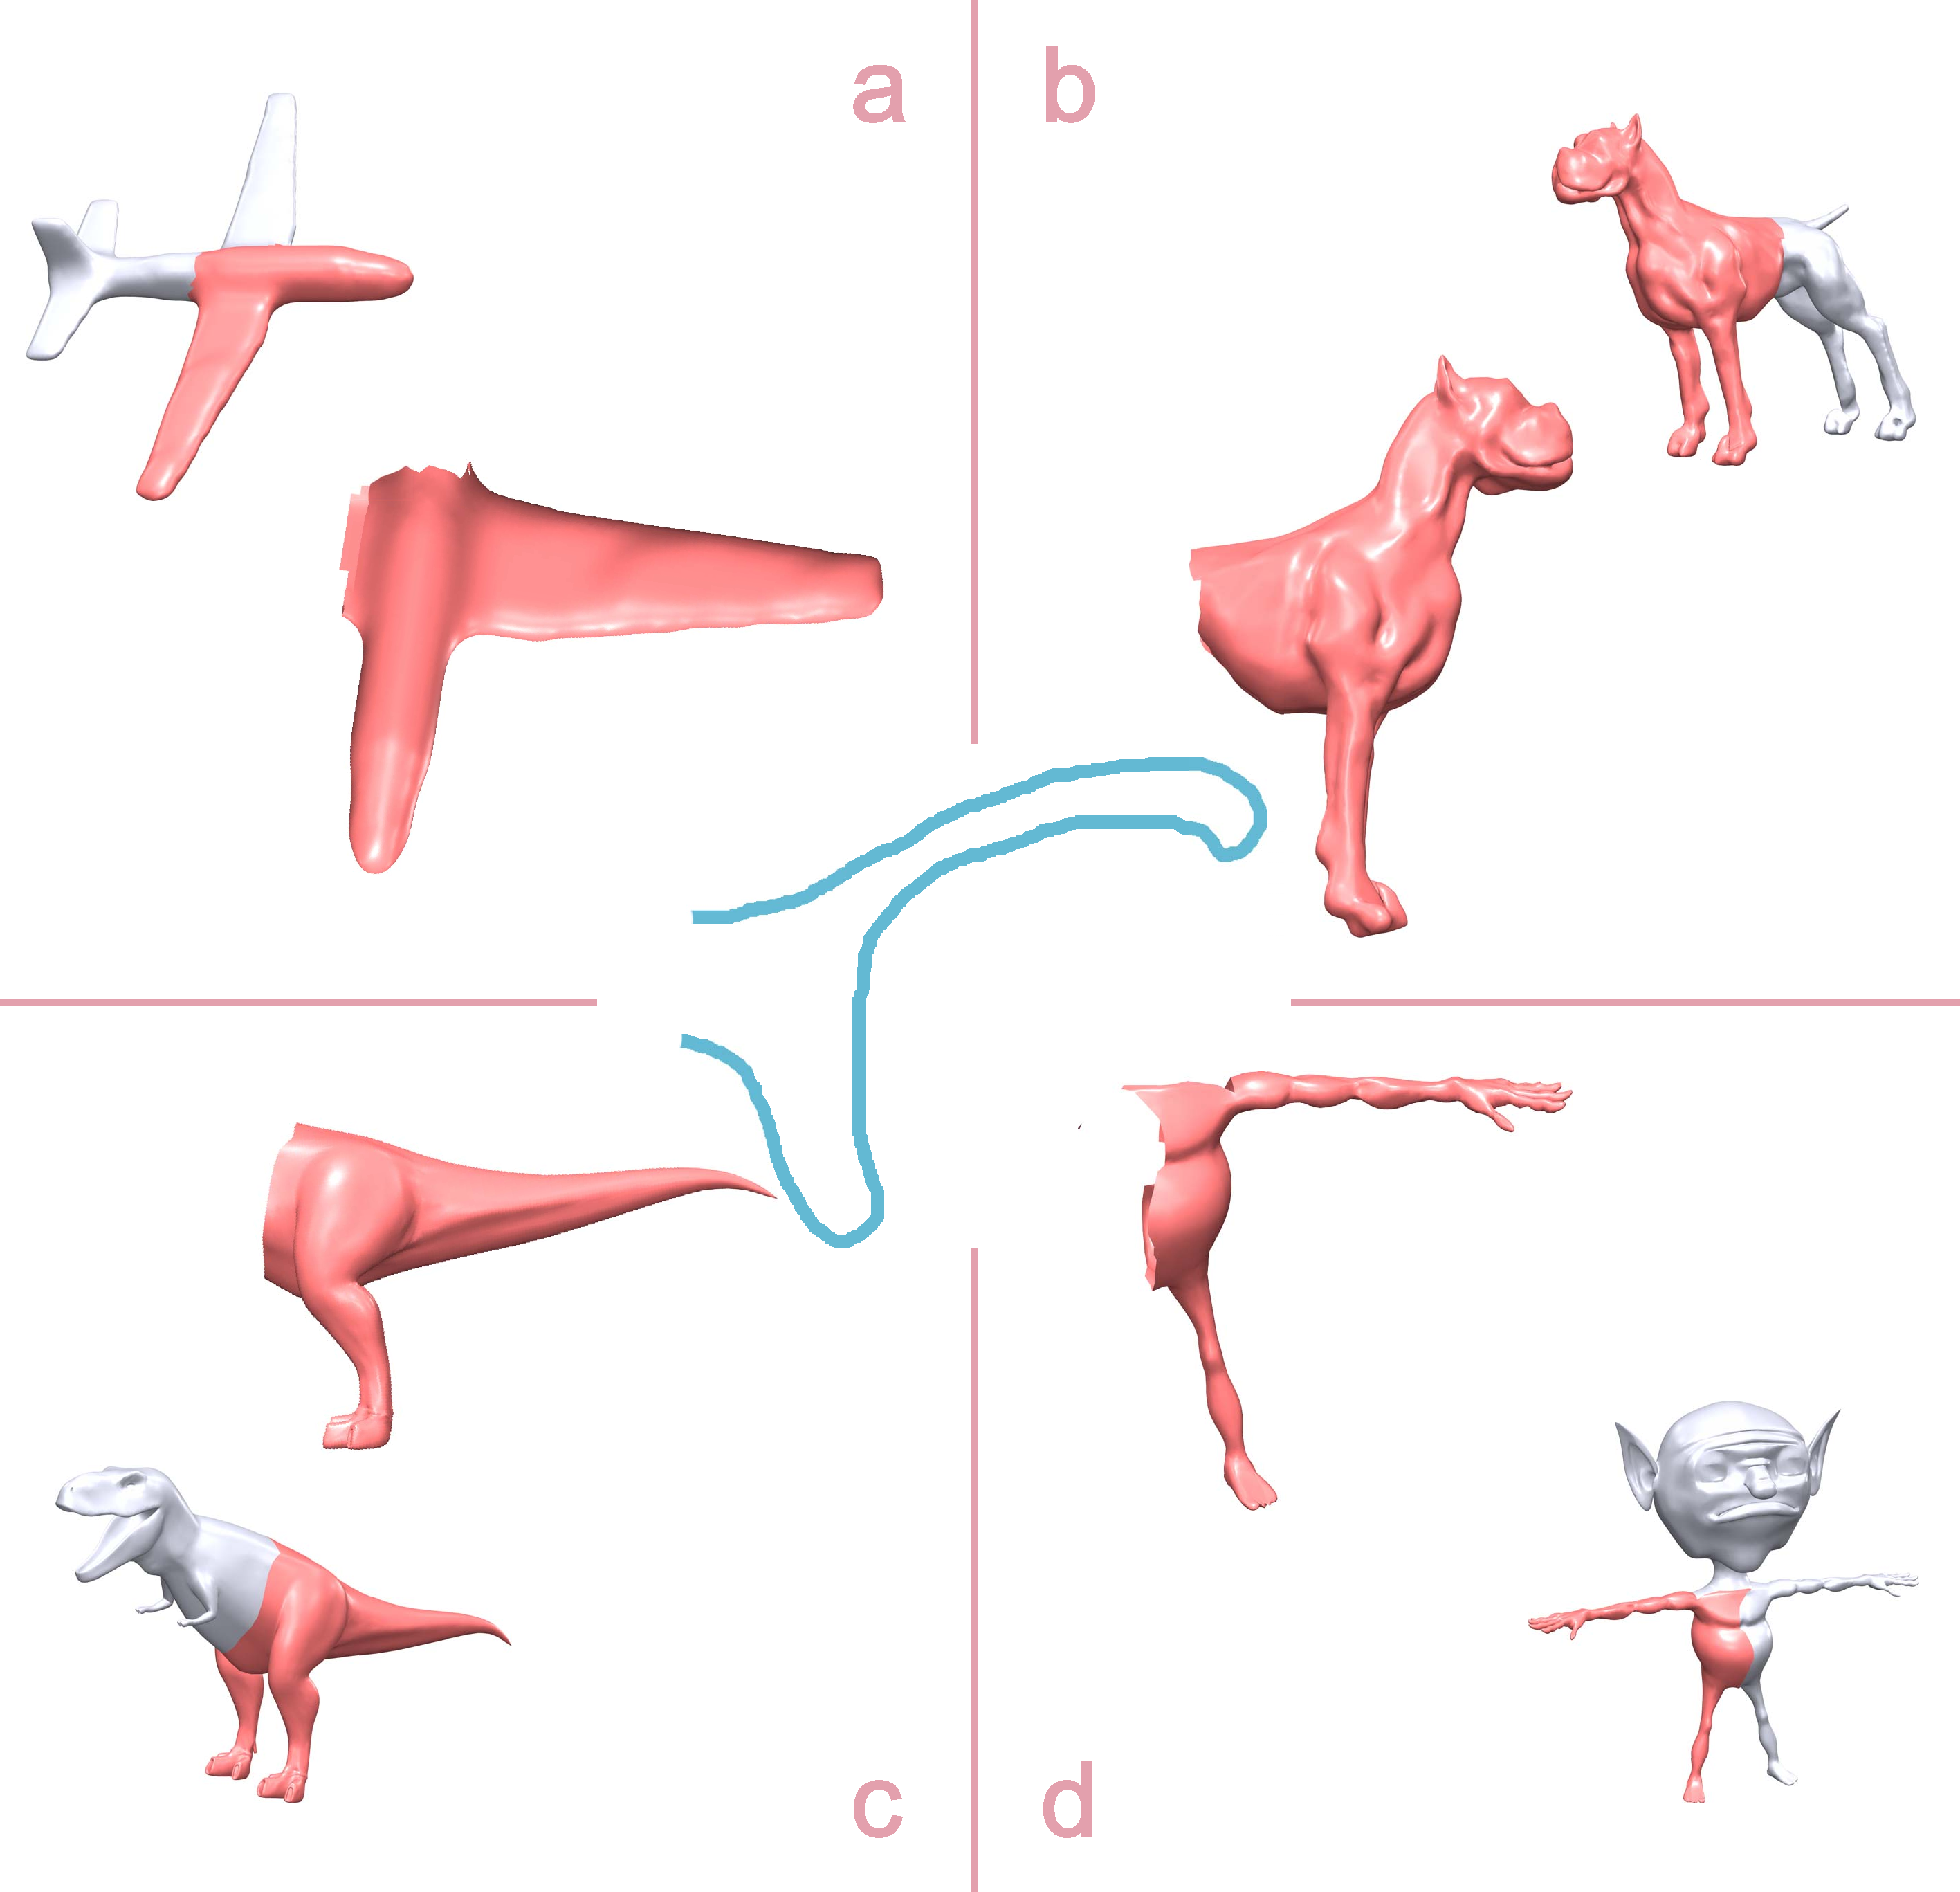
\includegraphics[width=0.9\linewidth]{./Material/TeaserSGP.pdf}
\caption{Given a roughly drawn sketch, our algorithm rapidly searches a shape database to identify and extract customized parts that match the sketch. No presegmentation is required: the retrieved parts can be irregular and not match any standard segmentation.}
\label{fig:HeadPic}
\end{figure}

\begin{figure*}[t]
\centering
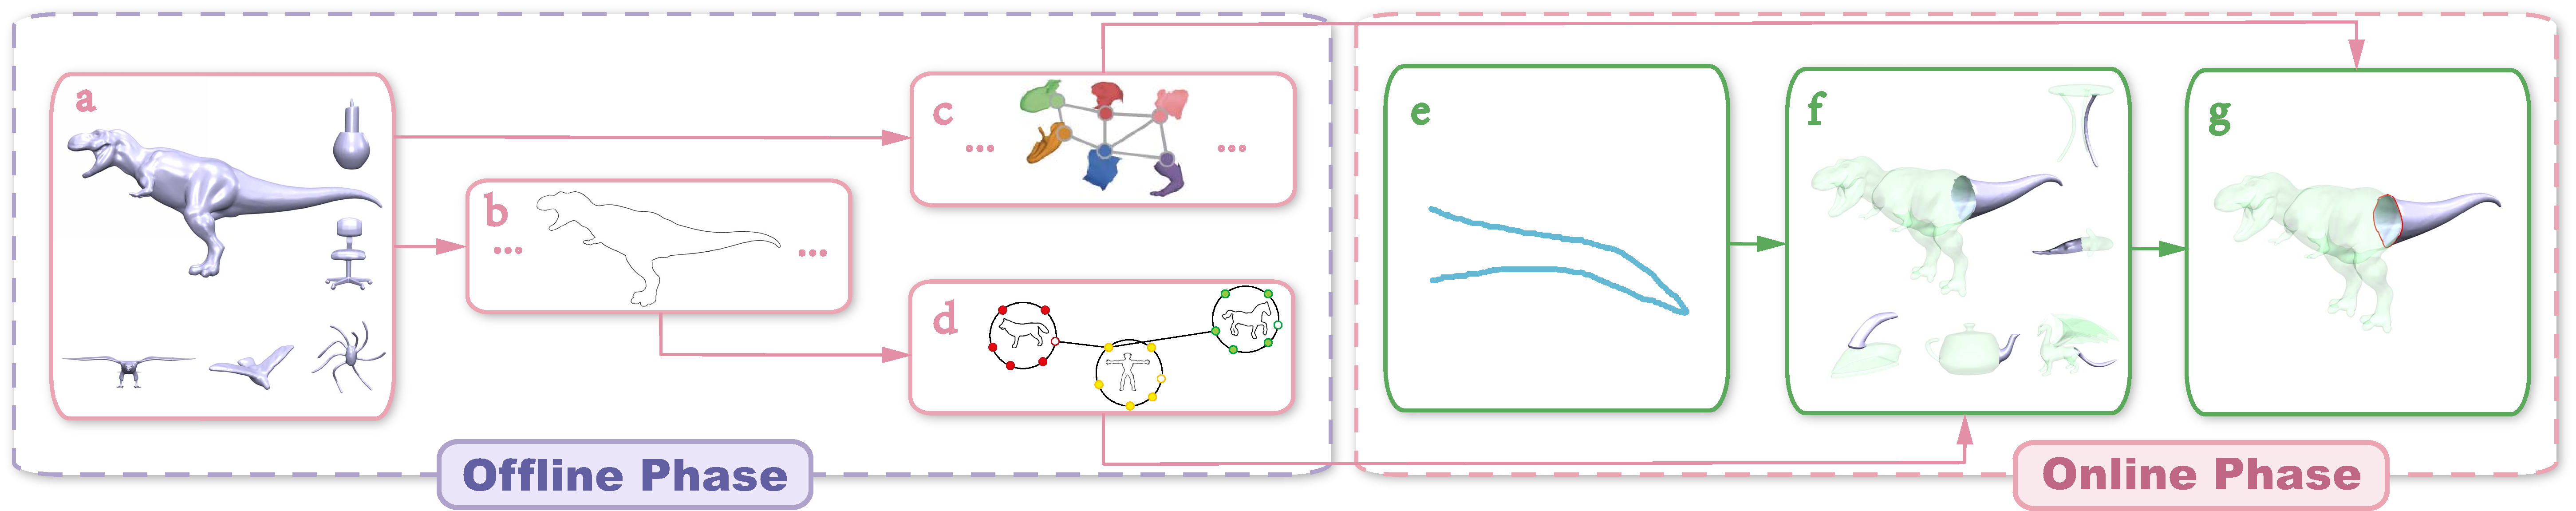
\includegraphics[width=\linewidth]{./Material/Pipeline.pdf}
\caption{Pipeline of our system. In the offline phase, for each model in a given shape database (a), we first extract its boundary contours (b). We then construct the \textbf{super-face graph} for each model (c), and organize the boundary contours of all models into a \textbf{randomized compound $k$-NN graph} (d). In the online phase, the user draws a rough sketch to convey his/her design intent (e). Regions of database shapes matching the sketch are rapidly identified via partial shape matching (f). A selected part is further refined to optimize its boundary and better match the sketch (g)}\label{fig:pipeline}
\end{figure*}

Matching a sketched component to a shape database is a challenging partial matching problem. In the general setting, an arbitrary region of the shape may match the sketch. To reduce the complexity, existing methods leverage a prior segmentation of each shape into predefined semantic parts~\cite{sketchbasedcompositionfunkhousersbim2008,sketchtodesignxukaicgf2013}. These parts are individually matched to the sketch, reducing the problem to one of global, rather than partial matching~\cite{EitRicBouHilAle12}.

In this paper, we present {\ProjName}, a new end-to-end technique for sketch-based customized part extraction. In contrast to prior work, we require no prior segmentation of the database shapes into predefined parts. Instead, we perform {\em on-demand} segmentation of retrieved database shapes, to accurately fit the user intent expressed in the sketched stroke (Figure \ref{fig:HeadPic}). This significantly expands the design space available to the user and enables several applications.

Designing such an algorithm presents hard technical challenges. Since a presegmented (or prelabeled) database is not available to us, we must simultaneously identify and extract parts that match sketched strokes, resulting in a potentially infinite search space. To prune this search space to a manageable size, we design a strategy to carefully balance between returning all possible matches, and providing an overly narrow set of matches. Further, the matching scheme must be fast enough so that appropriate candidate parts can be sought interactively. To address this challenge, we take a projective approach and turn the 3D partial matching problem into a 2D contour-based one. The 2D contours of all database shapes are segmented into fragments and organized based on fragment similarity, using an efficient data structure. Given a query sketch, our method can leverage the structure to quickly return all potentially matched parts via contour matching and match propagation.

Our paper has two main technical contributions, which together form the core of our algorithm:
\begin{itemize}
\setlength{\itemsep}{3pt}
\setlength{\parskip}{0pt}
\setlength{\parsep}{0pt}
\item A fast, sketch-based, partial 3D shape matching method based on multi-view projections. The projections are interlinked by matching fragments across different shapes, based on a novel randomized compound $k$-NN graph representation.
\item A novel customized segmentation method based on a super-face graph. The method quickly extracts candidate parts conforming to a user's sketch from a matched shape. The extraction employs a coarse-to-fine strategy to progressively refine part boundaries down to the level of individual faces.
\end{itemize}

%%%%%%%%%%%%%%%%%%%%%%%%%%%%%%%%%%%%%%%%%%%%%%%%%%%%%%%%%%%%%%%%%%%%%%%%%%%%%%%%%%%%%%%%%%%%%%%%%%%%%%%%%%%%
\section{Related work}
%%%%%%%%%%%%%%%%%%%%%%%%%%%%%%%%%%%%%%%%%%%%%%%%%%%%%%

\paragraph*{Sketch-Based Shape Retrieval.} With the rapid growth of 3D shape data, fast and convenient content-based shape retrieval techniques \cite{asurveyofcontentbasedtangeldermultimedia2008} have become important. Content-based methods usually require a user to provide a 3D shape as a query, which introduces a circular dependency in a 3D modeling scenario. In contrast, sketch-based methods \cite{asearchenginefunkhousertog2003,discriminativesketchbasedshaotianjiacgf2011,EitRicBouHilAle12} allow the user to roughly draw the outline of the desired shape from one or more viewpoints in 2D. This is typically a more intuitive and convenient way to describe the user's intention.

Lee and Funkhouser~\shortcite{sketchbasedcompositionfunkhousersbim2008} develop a sketch-based system for retrieving parts from a part database and incorporating them into a 3D model. Xie et al.~\shortcite{sketchtodesignxukaicgf2013} propose a similar system for shape editing by context-aware part replacement. These systems assume the parts are pre-generated by automatic segmentation, and hence retrieval reduces to global 2D-to-3D matching. The systems do not allow the user to generate new parts with novel cuts, or retrieve groups of pre-existing parts with one sketch. In contrast, our approach supports arbitrary cuts of exemplar shapes, driven by the sketch. Further, because shapes are not pre-segmented, we must do partial matching from 2D to 3D at interactive rates, which is a significant technical challenge.

%%%%%%%%%%%%%%%%%%%%%%%%%%%%%%%%%%%%%%%%%%%%%%%%%%%%%%

\paragraph*{Shape Segmentation.} Segmenting shapes into meaningful parts is a fundamental problem in many computer graphics tasks and applications, and both automatic and manual approaches have been developed to tackle this problem \cite{surveyonmeshsegmentationshamircgf2008,benchmarkforsegmentationchenxiaobaisg2009}. Recently, several groups have explored methods for jointly segmenting a set of shapes~\cite{learning3dmeshsegmentationkalosg2010,cosegmentationof3dshapesliuligangcgf2012,jointshapesegmentationhuangqixingsg2011,SidKaiKleZhaCoh11}. By considering a set of shapes as a whole, the segmentation can exploit shared structure and hence yield more coherent results. These works greatly benefit exploratory modeling systems by providing an automatically pre-segmented shape database for part suggestion and re-assembly.

In contrast to these systems, our approach does not assume a pre-segmented and pre-labeled shape database. Instead, we retrieve and segment shapes in real time based on a user sketch. Since, we cannot anticipate the exact boundary of the sketch, an on-the-fly and contour-aware segmentation method is required.

In contrast to sketch-based mesh cutting methods \cite{FanMeshCutting2012}, we do not know the source shape in advance, and we do not sketch directly on the source shape. Instead, we perform 2D-3D partial matching to automatically retrieve database shapes matching the query sketch.

%%%%%%%%%%%%%%%%%%%%%%%%%%%%%%%%%%%%%%%%%%%%%%%%%%%%%%

\paragraph*{Exploratory Shape Modeling.} The idea of incorporating creativity-inspiring exemplar elements into conventional conceptual modeling has been an active topic for the past few years.
%Generally, the core of creativity-supported modeling methods is to offer users the ability to efficiently explore all possible solutions.
Lee et al. \shortcite{LeeExampleGalleries2010} examine the efficicacy of using galleries of examples for creativity support during the design process.
%Talton et al.~\shortcite{TalGibYanHanKol09} described a data-driven approach to support the open-ended modeling of parametric shapes.
Chaudhuri et al.~\shortcite{datadrivenvladenaisa2010} mine a 3D shape database to suggest components to creatively extend a base shape, based on geometric compatibility. In subsequent work, the authors develop a statistical \st{models} \hl{model} of shape semantics to improve the suggestions~\cite{probabilisticreasoningvladlensg2011}. These works build upon the Modeling by Example system of Funkhouser et al.~\shortcite{modelingbyexamplefunkhousersg2004}, which allowed users to query shape databases with 3D proxies for novel parts.

%In parallel work, researchers have worked on automating the shape generation process, so the user directly explores a space of complete shapes. Talton et al.~\shortcite{TalGibYanHanKol09} describe a data-driven approach for exploring a high-dimensional space of parametric shapes. Xu et al.~\shortcite{setevolutionxukaisg2012} present a fit-and-diverse method for evolving a set of assembled shapes to match user intent. Kalogerakis et al.~\shortcite{aprobabilisticmodelvladlensg2012}, Averkiou et al.~\shortcite{AverkiouShapeSynth2014} and others describe generative probabilistic priors for shape synthesis.
%
%Our approach lies in the category of part-suggestion methods. However, the major technical contribution of our work is that we do not rely on a pre-segmented (or pre-labeled) database, and can generate arbitrarily shaped segments to perfectly match user sketches. Hence, our approach allows users to efficiently query a much larger design space. Our work also stands in contrast to Modeling by Example, since we construct proxies by 2D sketching, extract parts automatically, and do not require exemplar shapes to be co-aligned.

%%%%%%%%%%%%%%%%%%%%%%%%%%%%%%%%%%%%%%%%%%%%%%%%%%%%%%%%%%%%%%%%%%%%%%%%%%%%%%%%%%%%%%%%%%%%%%%%%%%%%%%%%%%%
\section{Overview}

The pipeline of our algorithm is illustrated in Figure \ref{fig:pipeline}. It consists of two phases: an \emph{offline phase} and \st{a} \hl{an} \emph{online phase}. In the offline phase, we construct acceleration structures critical for interactive on-demand part customization. In the online phase, we extract parts in response to user sketches.

\paragraph*{Offline Phase.}
First, we extract {\em boundary contours}~\cite{suggestivecontoursrusinkiewicztog2003} for each model in the database from different camera views. Then, we extract descriptors for the boundary contours at different scales (Section \ref{subsec:CtourDesc}).

Next, we organize all boundary contours of all models into a compound $k$-nearest neighbors graph, for fast retrieval (Section \ref{sec:acc}).

Finally, we construct a compact representation of each database shape: the super-face graph (Section \ref{subsec:sfg}). A super-face \hl{(analogous to superpixel}~\cite{RenLCM2003}\hl{)} is a group of adjacent, similar faces: factoring a shape into its super-faces yields a lower-complexity representation of the raw mesh. We use the super-face graph to quickly extract the part corresponding to a matched query contour.

\paragraph*{Online Phase.}
The input sketch is used to retrieve partially matching shapes (via the $k$-NN graph) and identify their regions matching the sketch (via the super-face graph). The boundary of each such region is optimized by a coarse-to-fine segmentation strategy: a rough boundary is first computed at the super-face level and then refined at the raw face level. In contrast to other methods \cite{surveyonmeshsegmentationshamircgf2008}, our segmentation method takes contour perception, concavity, and smoothness into consideration (Section \ref{sec:partrefinement}).

%%%%%%%%%%%%%%%%%%%%%%%%%%%%%%%%%%%%%%%%%%%%%%%%%%%%%%%%%%%%%%%%%%%%%%%%%%%%%%%%%%%%%%%%%%%%%%%%%%%%%%%%%%%%
\section{Data Structure for Fast Partial Matching}\label{sec:acc}

At runtime, the user sketches a desired part. The system rapidly searches the database to find parts matching the sketch. We support searching for arbitrarily shaped parts, not just those matching a ``standard'' presegmentation. Hence, we must process each database shape on the fly, identifying which section of the shape matches the sketch. This requires an extremely fast 2D-3D partial matching method.

To compare a 2D sketch to a larger 3D shape, we have two choices: (a) to infer a 3D proxy from the sketch \cite{Igarashi:1999:TSI:311535.311602} and match it to the shape, or (b) to compare the sketch to the 2D contours of the shape. We choose to do the latter for three reasons: (i) because it avoids the inherent ambiguity in inferring 3D shape from a 2D outline; (ii) because partial matching in 3D is significantly more expensive; and (iii) because the 2D sketch reflects the user's direct intent, which may be distorted when converting to 3D.

Therefore, we perform 2D partial matching between the sketch and multi-view projections of database shapes. In the offline phase, we render and store boundary contours of each database shape from a large number of camera views. Then, the problem reduces to matching the sketch to a section of one of these exemplar contours.

\begin{figure}[t]\centering
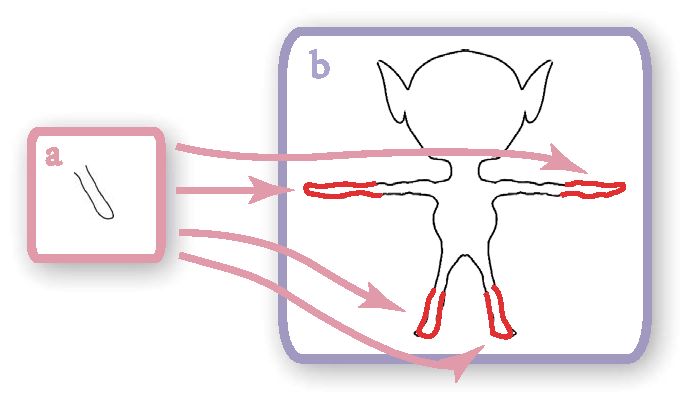
\includegraphics[width=0.85\linewidth]{./Material/CtourMatch.pdf}
\caption{A single contour may match a query contour in more than one section. The shape contour (b) matches the query contour (a) in four different sections (marked in red).}\label{fig:CtourMatch}
\end{figure}

It is a significant challenge to quickly search the huge set of exemplar contours for sections that match the sketch. Existing algorithms such as partitioning trees~\cite{scalablenearestmujapami2014}, hashing~\cite{nearoptimalandoniacm2008}, and $k$-nearest neighbor graphs~\cite{scalableknnjingwangcvpr2012} are designed for global, not partial matches.

To rapidly find database shapes whose contours match the sketch, we propose a new data structure: the {\em Randomized Compound $k$-Nearest Neighbors Graph} ({\RCKNNG}). The {\RCKNNG} has as its vertices all rendered contours of all database shapes. In a standard $k$-nearest neighbor graph~\cite{scalableknnjingwangcvpr2012}, each contour would be connected to its $k$ most similar neighbors. This information is used to quickly retrieve new matches once an initial positive match is found.

In our partial matching scenario, however, a single contour may match a query contour in more than one section, as illustrated in Figure \ref{fig:CtourMatch}. To reflect this, the {\RCKNNG} allows a contour to be connected to several different sets of $k$ neighbors. Each such set corresponds to a different matched section. Thus, from a partial match in one shape, we can quickly find several other partial matches with similar geometry in other shapes.

\begin{figure}[t]\centering
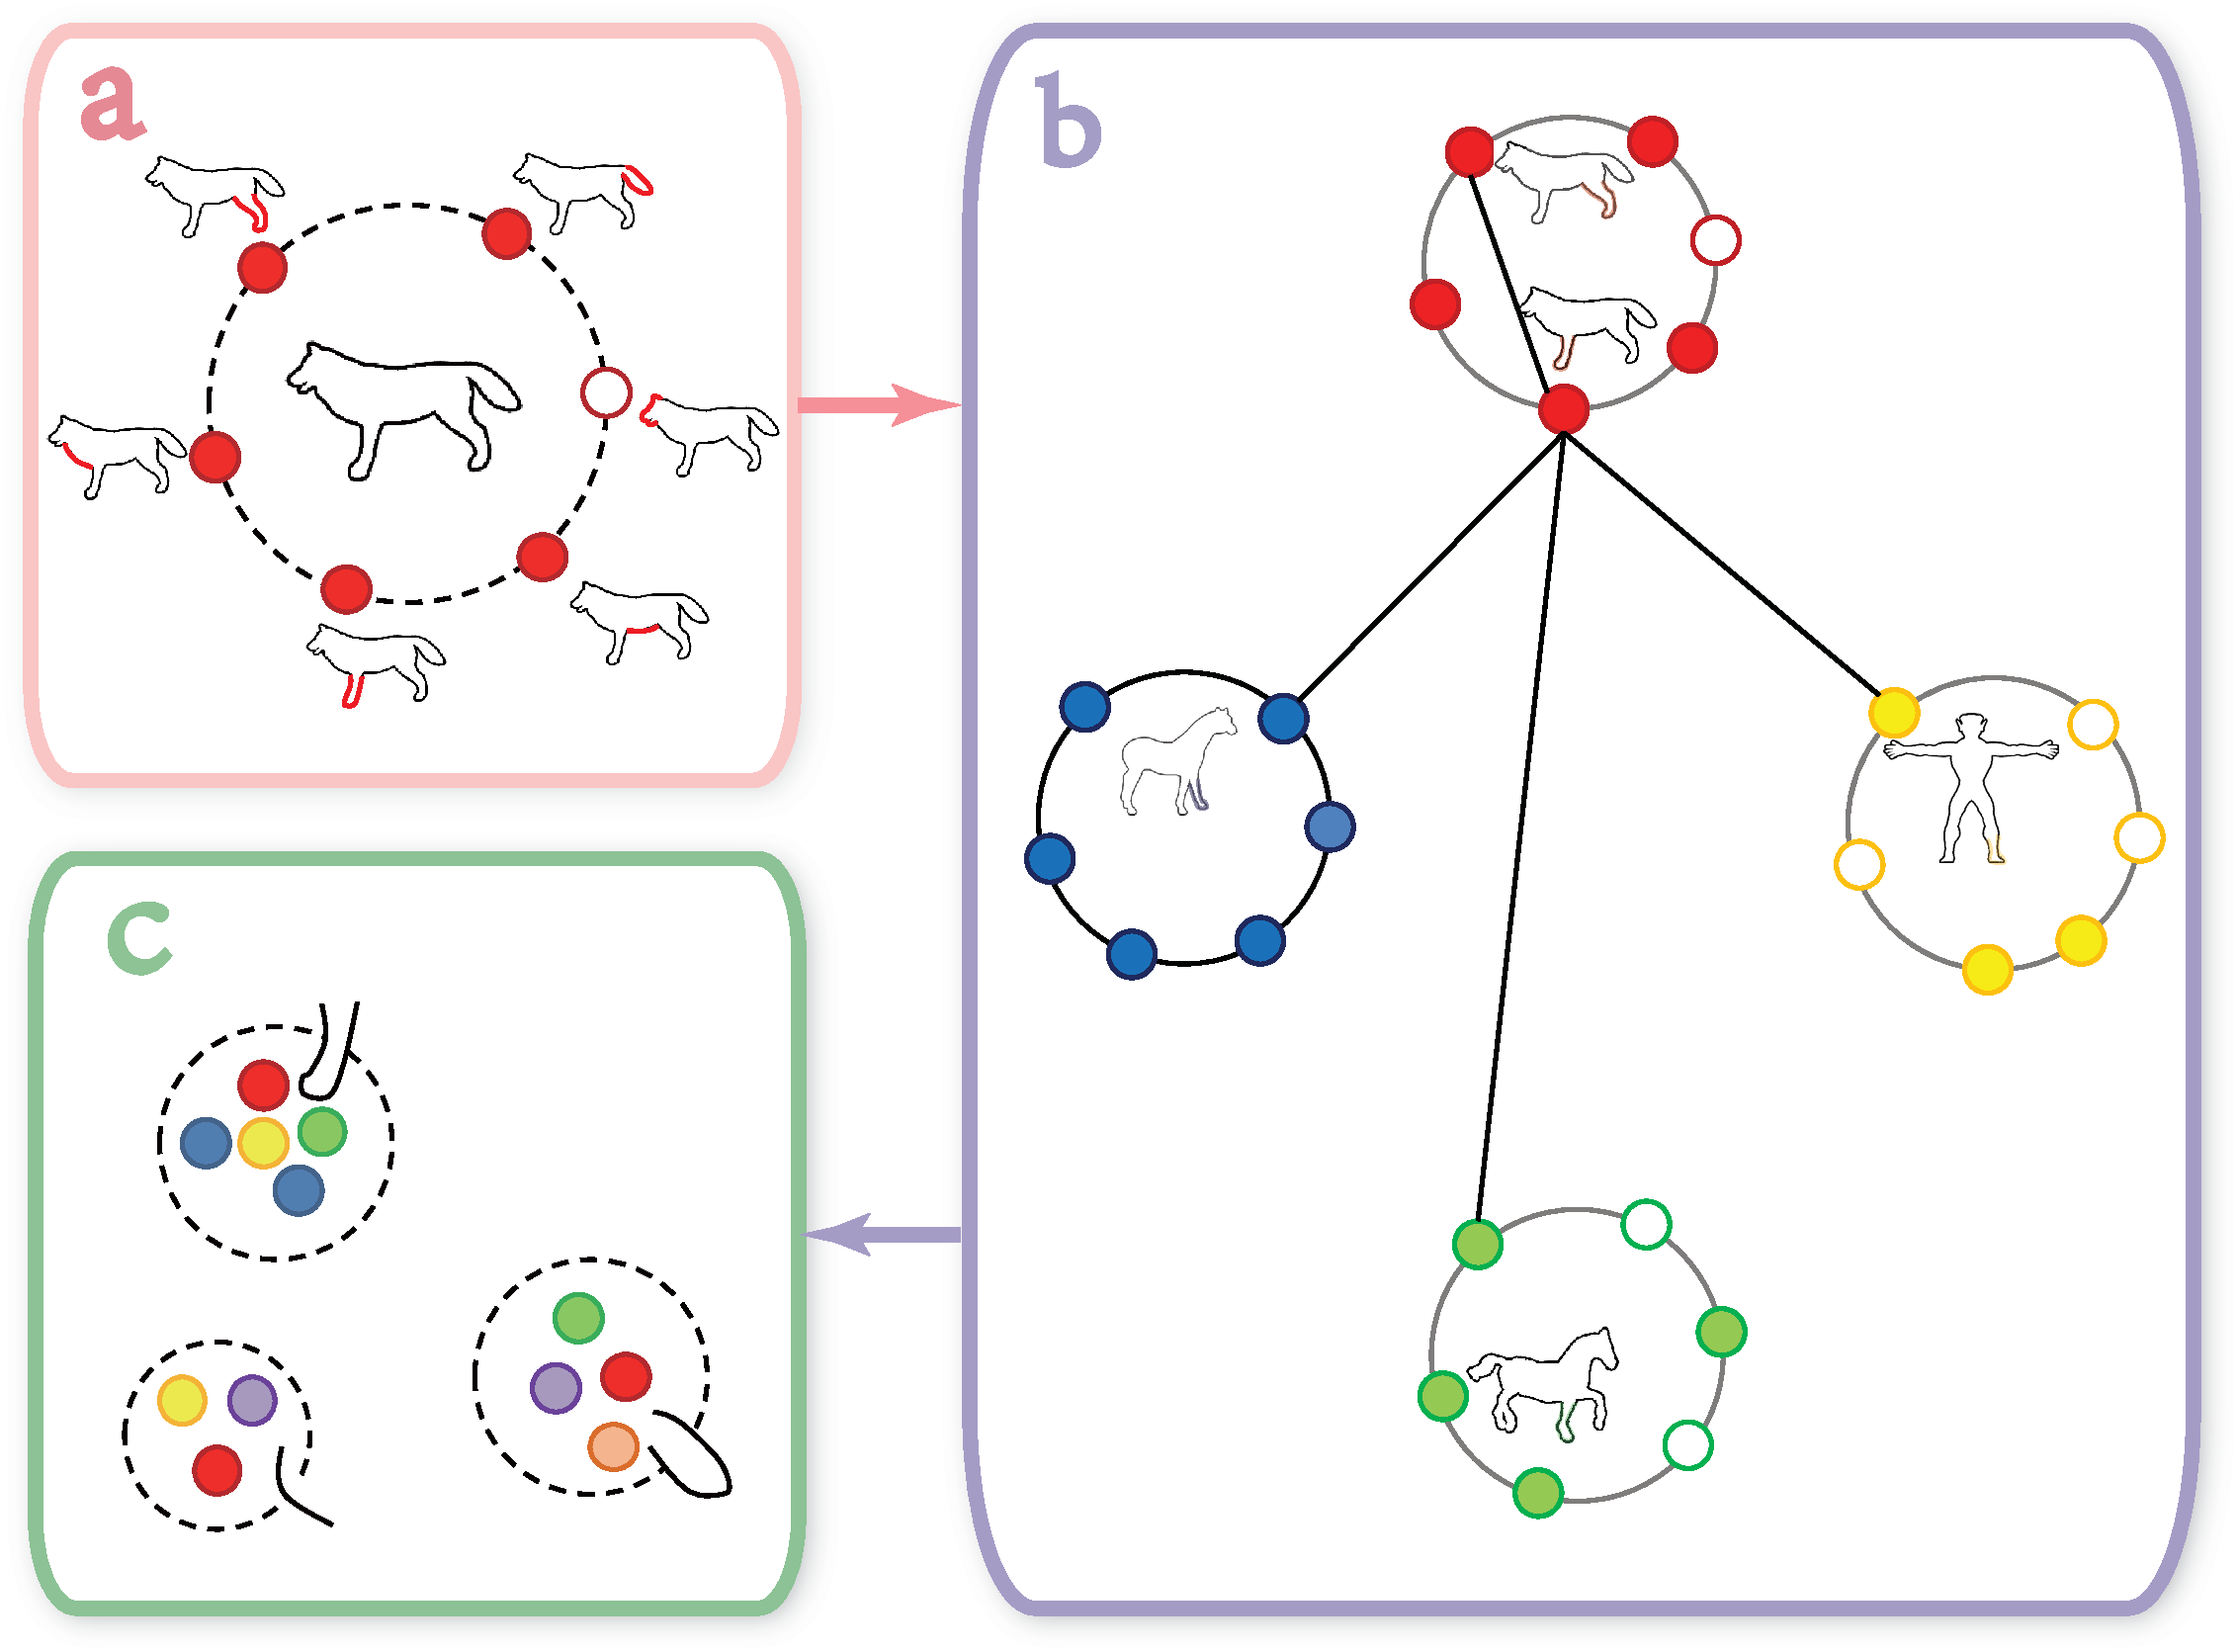
\includegraphics[width=1.0\linewidth]{./Material/KNN.pdf}
\caption{Illustration of our randomized compound $k$NN graph. In this figure, a solid circle represents a valid section and a dashed circle represents an invalid one. Given a contour (taken as a node of our randomized compound $k$NN graph), we first generate several sections (a). Then, we find the nearest neighbors for each section and establish edges between the parent contours of these sections (b). Finally, we find valid sections and cluster them (c).}\label{fig:KNN}
\end{figure}

\paragraph*{Construction of the {\RCKNNG}.} Direct construction of the compound $k$NN graph by exhaustively comparing all possible sections of all pairs of contours is prohibitively expensive. Instead, we choose to approximate the graph with a double-random strategy:
%
\begin{enumerate}
  \item We first generate $n$ sections (we use $n=6$ in our experiments) from each contour at each scale (Figure \ref{fig:KNN} (a)). A scale level comprises uniformly spaced points along the contour: a higher level has smaller spacing and hence a larger overall number of points. Our levels place $50$, $150$ and $250$ points along the contour respectively.

To generate a section, we randomly choose an uncovered point with a probability $p$ proportional to its curvature $c$ and distance $d$ to the nearest point covered by other sections: $p \propto c \cdot d$. The section then covers \st{$m = 20$} \hl{$m = 21$} consecutive points with the selected point at the center.

  \item We adopt a multiple random divide-and-conquer strategy~\cite{scalableknnjingwangcvpr2012} to construct a $k$NN graph of all the sections (Figure \ref{fig:KNN} (b)).
\end{enumerate}
%
We collect all ``valid'' sections into a global list. A section is considered valid when the distance (which will be defined in Section \ref{subsec:CtourDesc}) between it and each of its $k$ nearest neighbors is below a threshold $\varepsilon=0.85$. After that, we cluster the \hl{global} list to get a sparse set of sections (the cluster centers) which will be used as seed points for queries (Figure \ref{fig:KNN} (c)). \hl{The clustering is based on the same distance defined in Section } \ref{subsec:CtourDesc}. The number of clusters is empirically set to $1708$.
%


%%%%%%%%%%%%%%%%%%%%%%%%%%%%%%%%%%%%%%%%%%%%%%%%%%%%%%%%%%%%%%%%%%%%%%%%%%%%%%%%%%%%%%%%%%%%%%%%%%%%%%%%%%%%
\section{Candidate Shape Retrieval}\label{sec:candshape}
%%%%%%%%%%%%%%%%%%%%%%%%%%%%%%%%%%%%%%%%%%%%%%%%%%%%%%
In this section, we describe how the {\RCKNNG} is used to quickly and accurately retrieve candidate parts that match the sketch, from an unsegmented database.

\subsection{Contour Descriptor}\label{subsec:CtourDesc}
Each contour is divided into sections. The query contour, which is the sketch, has a single section. Database shape contours have several sections at each scale (Section \ref{sec:acc}), each of which may resemble the query to yield a partial match.

To compare two contour sections, we generate contour descriptors. The particular descriptor we employ is a matrix of angles~\cite{partialedgecontourriemeneccv2010}. The descriptor is calculated from the relative spatial orientations of lines connecting sampled points on the contour.

A section of a contour has \st{$m = 20$} \hl{$m = 21$} sampled points on it. For each pair of points $(b_i, b_j)$, we compute an angle metric $\alpha_{ij}$:
\[{\alpha _{ij}} = \left\{ {\begin{array}{*{20}{c}}
   {\left\langle {\overline {{b_i}{b_j}} ,\overline {{b_i}{b_{i + \Delta }}} } \right\rangle } & {\text{if~} i < j,}  \\
   {\left\langle {\overline {{b_i}{b_j}} ,\overline {{b_i}{b_{i - \Delta }}} } \right\rangle } & {\text{if~} i > j,}  \\
   0 & {\text{if~} \left\| {i - j} \right\| \le \Delta }  \\
\end{array}} \right.\]
where $\Delta = 2$ is an offset parameter and $\langle \ell_1, \ell_2 \rangle$ denotes the angle between lines $\ell_1$ and $\ell_2$. The contour descriptor is then the angle matrix $A$, where $A_{ij} = \alpha_{ij}$. The distance between two contour sections $S$ and $T$ is the squared Euclidean distance between their angle matrices $A^S$ and $A^T$:
\[
D(S, T) = \frac{1}{m^2} \sum_{i = 1}^m \sum_{j = 1}^m \left( A^S_{ij} - A^T_{ij} \right)^2
\]

%%%%%%%%%%%%%%%%%%%%%%%%%%%%%%%%%%%%%%%%%%%%%%%%%%%%%%
\subsection{Shape Retrieval}
We need to identify $c$ partially matching shapes from which candidate parts will be presented to the user (our experiments use $c = 9$). To achieve this, we query the ${\RCKNNG}$ for a larger number ($21c$) of matching contour sections, and compute a score for each parent shape. The $c$ shapes with highest scores are presented in the interface.

To generate the pool of contour sections, we first compare the query contour to all seed sections in the ${\RCKNNG}$. The results are sorted in a priority queue according to increasing descriptor distance, allowing us to traverse the graph in a best-first manner. The current best matching section is at the top of the queue. When it is popped off, its neighbors are compared to the query and added to the queue if they are not already there. We continue until we have popped and stored $21c$ matching sections.

A shape with at least one section in the matched pool is assigned the following score, which is used to rank the shapes for selecting the final candidates:
\[
s = \frac{\alpha }{t}\sum\limits_{i = 1}^t {{D_i}}  + \frac{\beta }{t},
\]
where $t$ is the number of matched sections in the shape contour, and $D_i$ is the distance of the $i^{\textrm{th}}$ matched section's descriptor from the query. We empirically set $\alpha = 0.95$, $\beta = 0.05$.


%%%%%%%%%%%%%%%%%%%%%%%%%%%%%%%%%%%%%%%%%%%%%%%%%%%%%%%%%%%%%%%%%%%%%%%%%%%%%%%%%%%%%%%%%%%%%%%%%%%%%%%%%%%%
\section{Progressive Part Extraction}\label{sec:partextraction}
When a user selects a candidate shape with a contour section matching the sketch, we must quickly and accurately identify and extract the corresponding part. This presents several challenges:
%
\begin{itemize}
\item A single contour may cover more than one semantic part. By ``semantic part'', we mean one that is typically identified by human labeling or a traditional segmentation algorithm, such as the head of an animal or the back of a chair.
\item The contour boundary may be irregular and not directly correspond to a semantic part boundary. Hence, it can be identified only with reference to the user's sketch.
\item The segmentation process should run at interactive speeds.
\end{itemize}
%
The first two scenarios are illustrated in Figure \ref{fig:partseg}.
%
\begin{figure}\centering
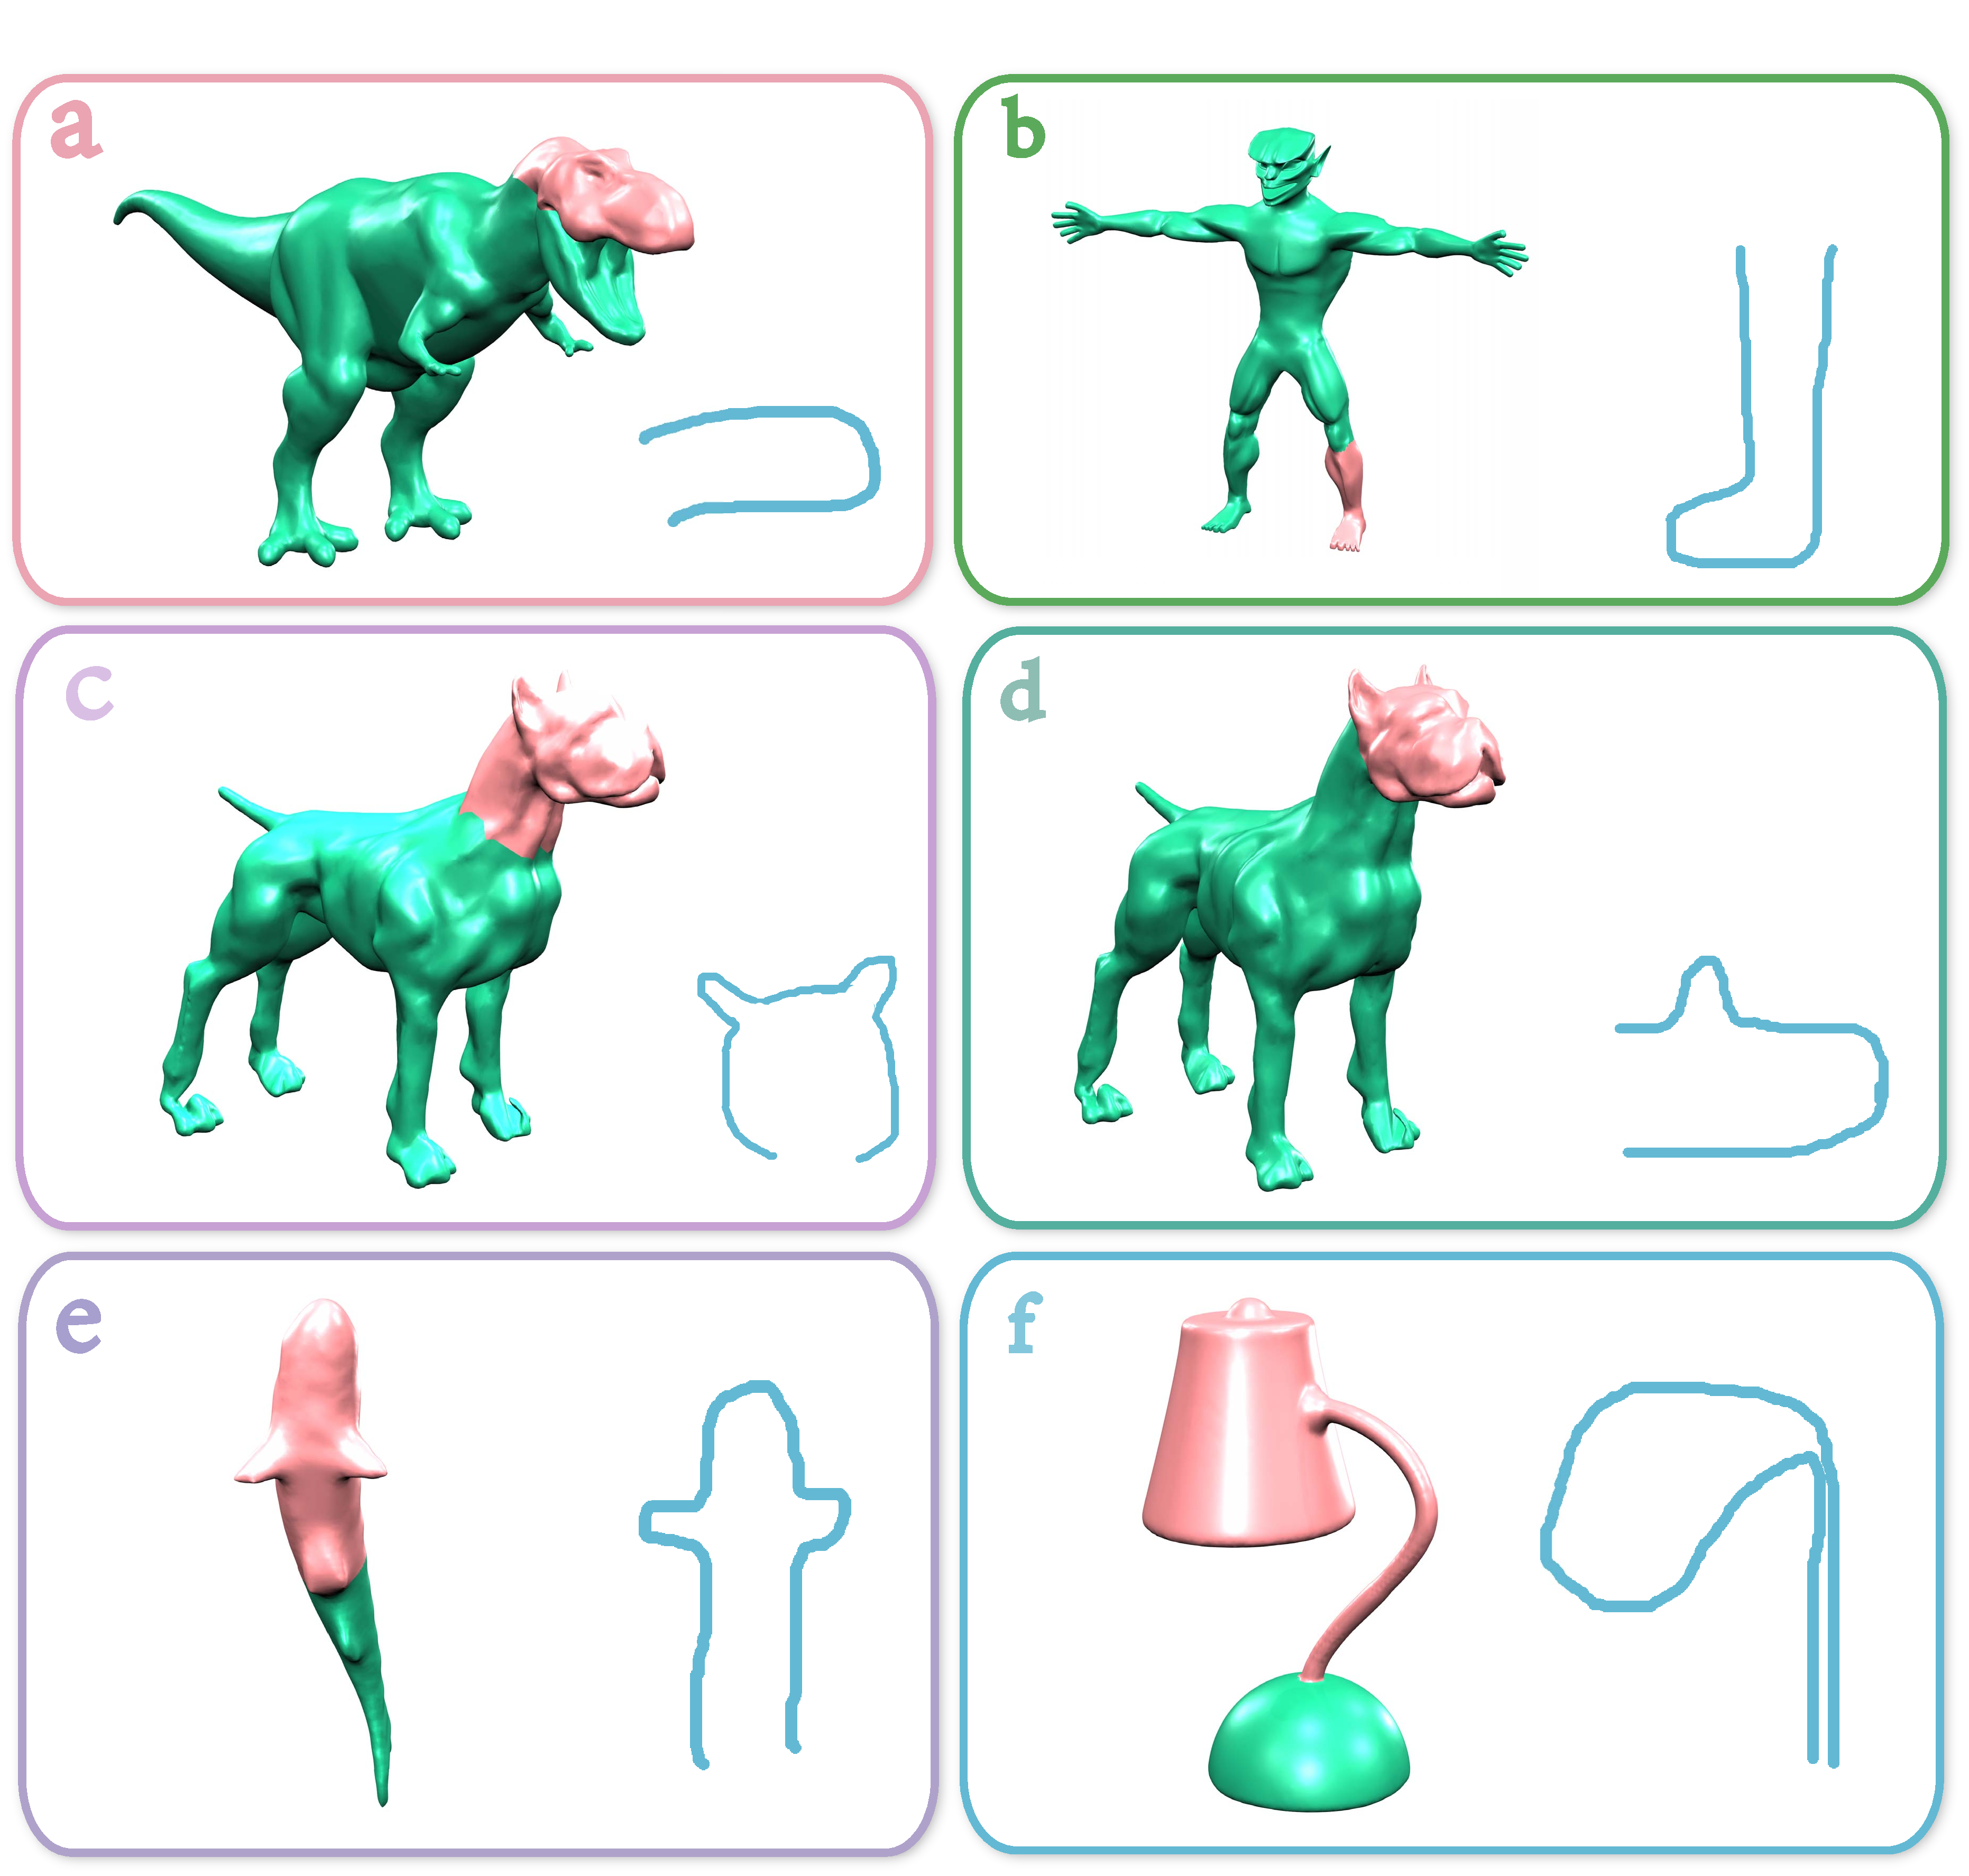
\includegraphics[width=\linewidth]{./Material/IrreWay.pdf}
\caption{Different types of parts (red) retrieved by a sketch (blue) using our algorithm. While some parts may be predefined with an automatic segmentation algorithm (d), others are irregular, defined only by the sketch (a,e), and yet others combine multiple ``standard'' segments (b: shin + foot, c: head + neck, f: shade + neck).}\label{fig:partseg}
\end{figure}

We address these challenges with a new \emph{super-face graph representation} (SFG) for a 3D shape. The super-face graph is a discretized yet fine-grained version of the original model. The vertices of the graph are a set of super-faces, obtained by an oversegmentation of the model that respects strong feature boundaries. While we could also work with the raw faces of the model, their combinatorial search space can be infeasibly large. Hence, we find candidate parts as combinations of super-faces, and subsequently refine the part boundaries down to the level of individual faces (Section \ref{sec:partrefinement}).

Edges of the graph connect pairs of adjacent super-faces. The weight of an edge indicates how frequently the super-face pair co-occurs in a single segment produced by a randomized segmentation algorithm (Figure \ref{fig:SFG}).

\begin{figure}[b]\centering
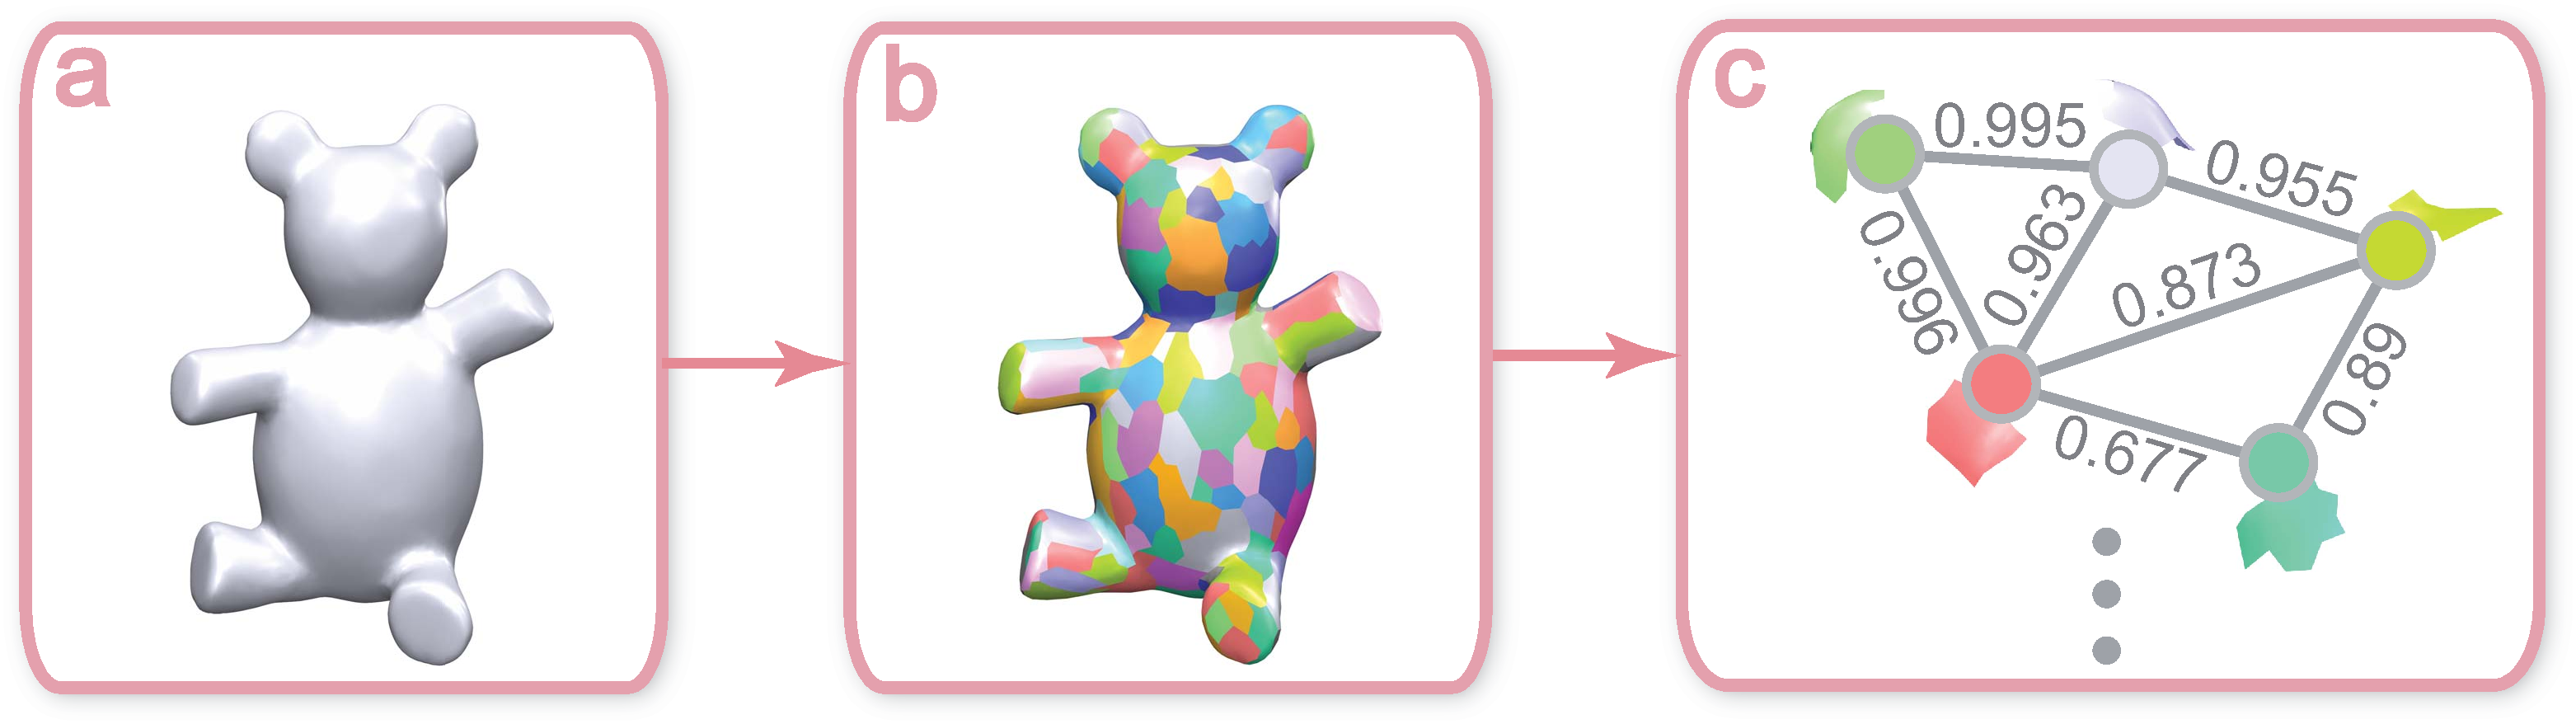
\includegraphics[width=\linewidth]{./Material/SFG.pdf}
\caption{The construction of the super-face graph for a 3D shape. Given the Teddy model (a), we partition it into a large number of super-faces (b). Each super-face is a node of the graph. Adjacent super-faces are connected by a weighted graph edge (c).}\label{fig:SFG}
\end{figure}

The super-face graph gives us a probabilistic prior for merging adjacent superfaces into larger patches to represent an arbitrary but not implausible or disconnected part of the shape. We generate the super-face graph representations of all database models in the offline phase.

%%%%%%%%%%%%%%%%%%%%%%%%%%%%%%%%%%%%%%%%%%%%%%%%%%%%%%
\subsection{Super-Face Graph Representation}\label{subsec:sfg}

To construct the super-face graph for a shape mesh, we oversegment the mesh into $N$ patches~\cite{jointshapesegmentationhuangqixingsg2011} (we experimented with $N = 50$, $100$ and $200$) and take each patch as a super-face (a vertex of the graph). Each pair of adjacent super-faces is connected by a graph edge.

\begin{figure}[b]\centering
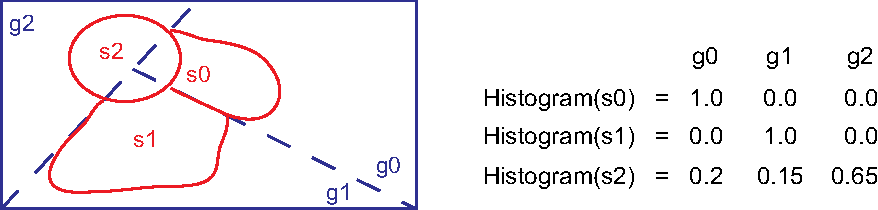
\includegraphics[width=1.0\linewidth]{./Material/Consistency.pdf}
\caption{Distributions of super-faces on segments. $s_0$, $s_1$, and $s_2$ are the super-faces. $g_0$, $g_1$, and $g_2$ are the segments generated by the randomized segmentation on the shape.}\label{fig:Consistency}
\end{figure}

To compute edge weights between nodes, we generate $900$ randomized segmentations~\cite{randomizedcutsfunkhousertog2008} over the shape with the number of segments varying from $2$ to $10$. Given a segmentation, we construct a histogram for each super-face, describing its segment memberships. Each bin of the histogram corresponds to a segment, and the value of the bin is the fractional area of the super-face lying within the segment (Figure \ref{fig:Consistency}). Mathematically, the bin value $h_s^g$ of a super-face $s$, for a segment $g$, is defined as:
\[h_s^g = \frac{{\sum\limits_{f ~\in~ Faces(g) \cap Faces(s)} {Area\left( {f} \right)} }}{{\sum\limits_{f ~\in~ Faces(s)} {Area\left( {f} \right)} }},\]
%\[h_s^g = \frac{{\sum\limits_{f \in Faces\left( g \right) \cap Faces\left( s \right)} {Area\left( f \right)} }}{{\sum\limits_{f \in Faces\left( s \right)} {Area\left( f \right)} }},\]
where $Faces(x)$ is the set of mesh faces in $x$, and $Area(f)$ is the area of face $f$.

These histograms serve as feature vectors for determining the probability that two super-faces may lie in the same segment. We define $P(s,s')$ as the probability that two adjacent super-faces $s$ and $s'$ lie in the same segment, and it is defined via the ${\chi ^2}$ distance between their histograms $H$ and $H'$:
\[{P}\left( {s,s'} \right) = 1 - {\chi ^2}\left( {H,H'} \right) = 1 - \frac{1}{2}\sum\limits_{{g_i} \in G} {\frac{{{{\left( {h_s^{{g_i}} - h_{s'}^{{g_i}}} \right)}^2}}}{{{{\left( {h_s^{{g_i}} + h_{s'}^{{g_i}}} \right)}^2}}}}, \]
where $G = \left\{ {{g_i}\left| {1 \le i \le N} \right.} \right\}$ is the set of segments generated by the randomized segmentation, $g_i$ is the $i$th segment, and $N$ is the number of segments.

To calculate the edge weight between two adjacent super-faces, we first accumulate the consistency scores over all the different randomized segmentations, and then normalize it using the number of randomized segmentation operations.

%--------------------------
\subsection{Fuzzy Part Identification}
As a first step, we use the SFG to extract a rough approximation of the part corresponding to a matched contour section. We can convert an open section to a closed one by drawing a line between its ends. This forms a natural perceptual boundary for the projection of the desired part.

Now, we start with any super-face adjacent to the center of the contour and perform a flood fill, gathering all super-faces whose projections lie within the closed contour obtained above.

We must handle several complications here. First, the contour section may be depth-discontinuous, spanning multiple isolated parts in 3D (Figure \ref{fig:ComplexCtour}(a)). Second, the contour section may enclose empty space that is not accounted for in the sketch (the blue and green sections in Figure \ref{fig:ComplexCtour}(b)). Third, the same sketch may match multiple instances of the same part (Figure \ref{fig:ComplexCtour}(c)). To address these issues, we filter out invalid parts and collapse multiple instances into a single part. \hl{The invalid parts generated with depth-discontinuous contour sections are identified by a group of isolated super-faces. This kind of parts are discarded. The multiple instances of the same part (Figure }\ref{fig:ComplexCtour}\hl{(c)) are identified by matching the sets of the super-faces. The repetitive instances are removed.}

\begin{figure}\centering
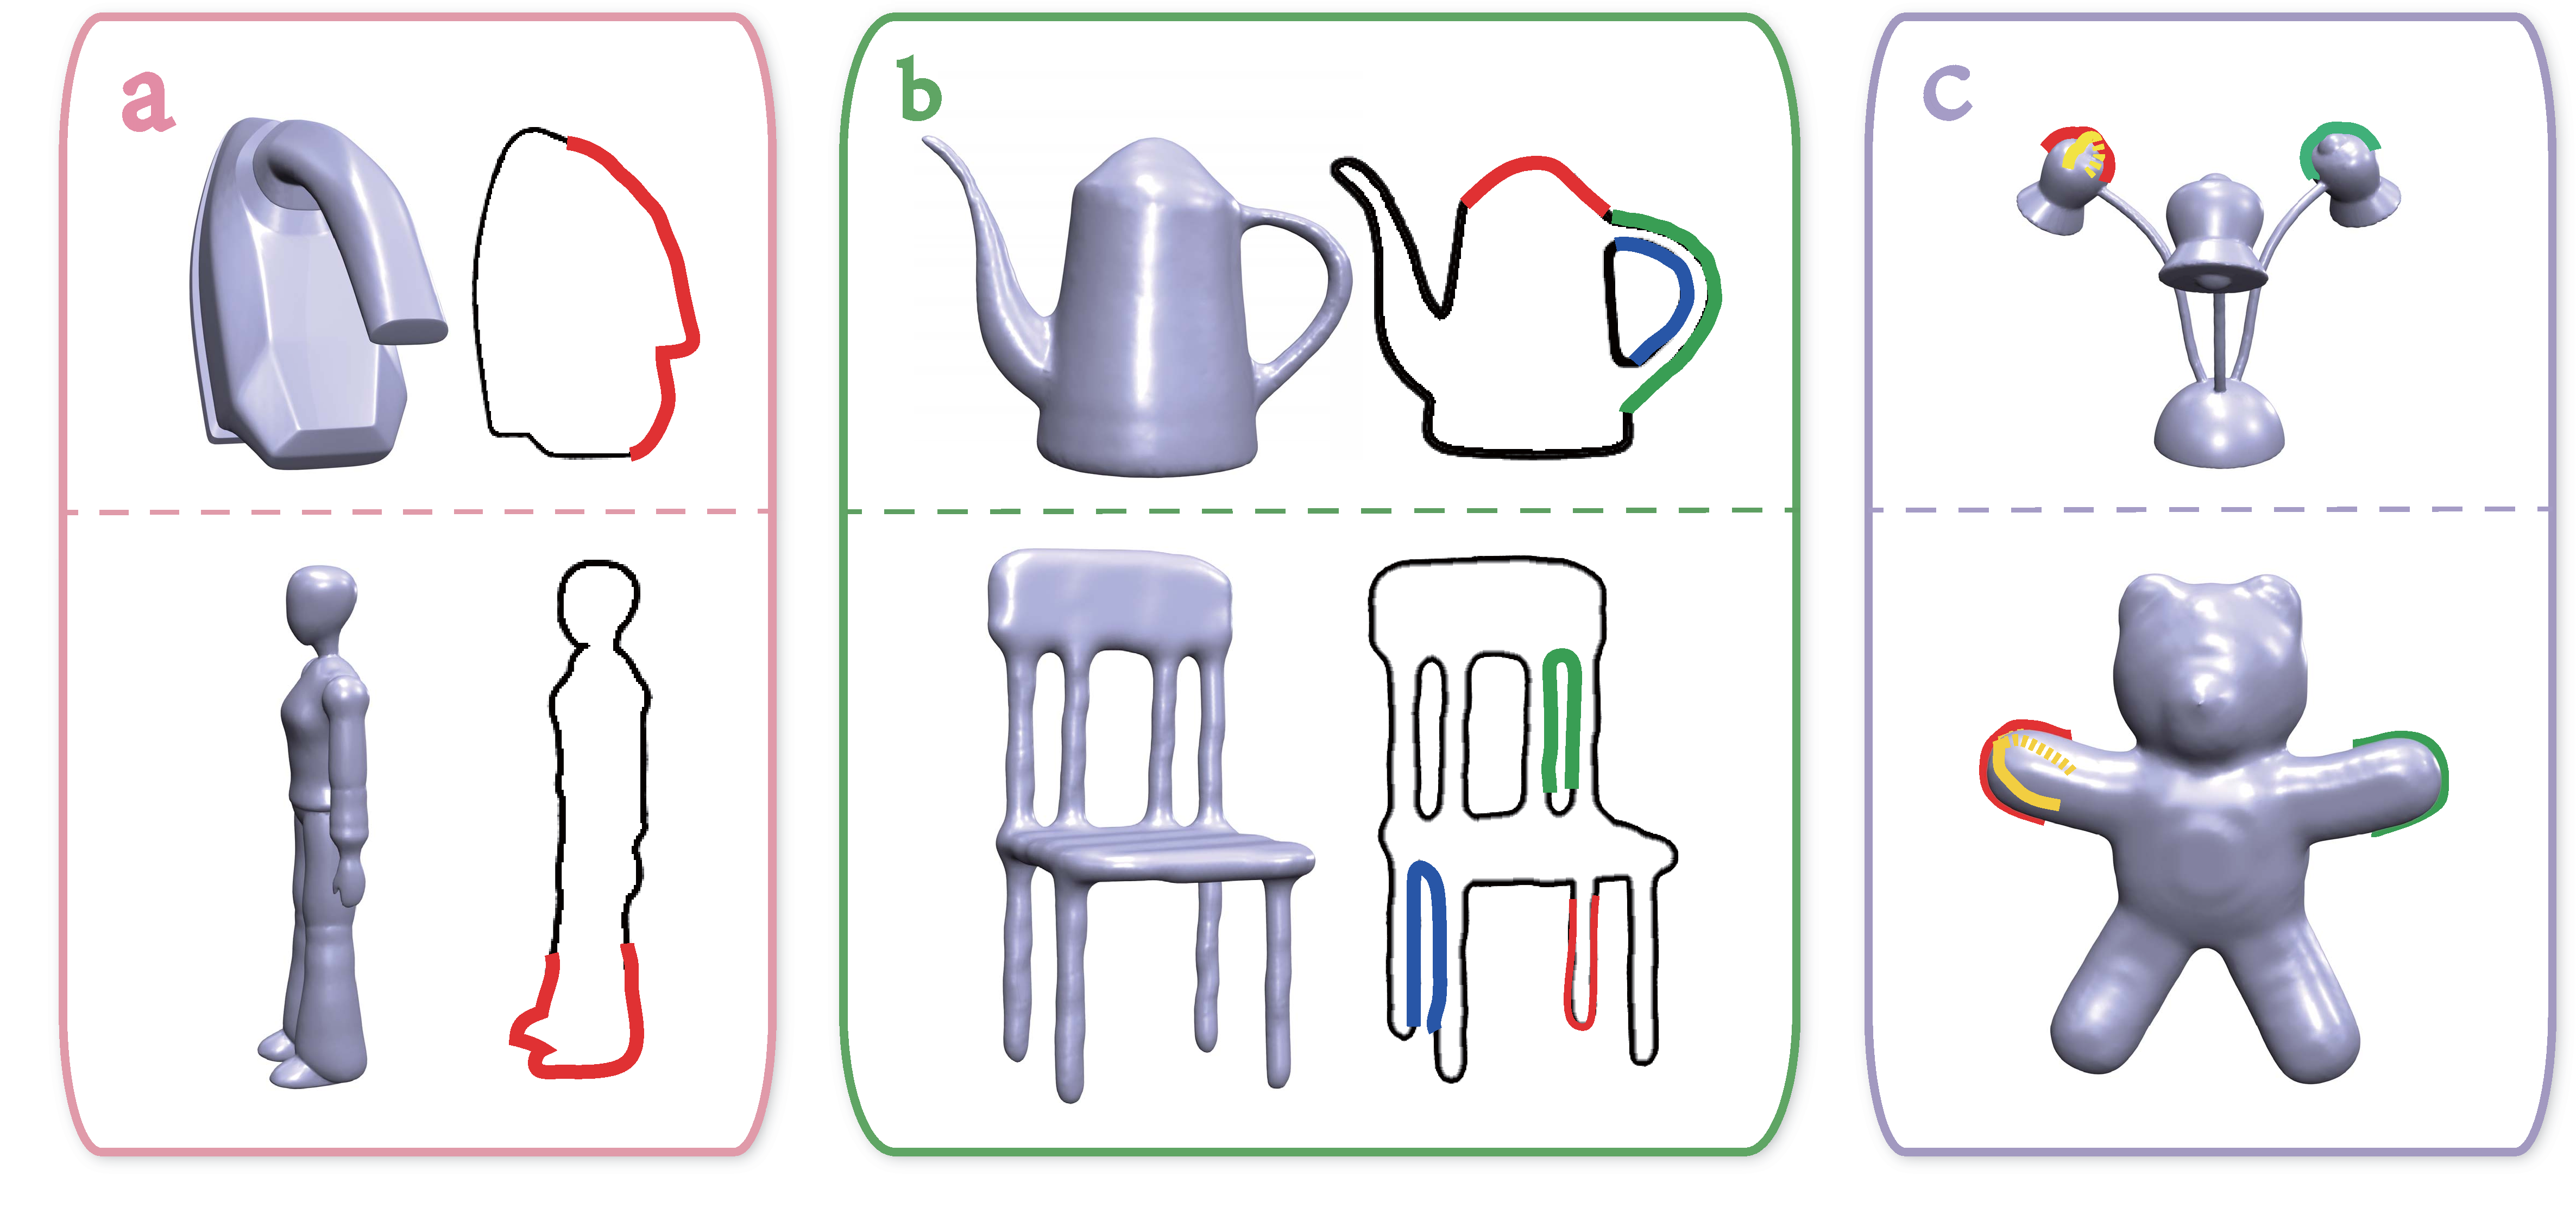
\includegraphics[width=\linewidth]{./Material/ComplexCtour.pdf}
\caption{Illustrations of the complexity of contours and their relationship. Depth-discontinuous contour sections are shown in (a). Topologically different contour sections are illustrated in (b). Isolated contour sections are shown in (c).}\label{fig:ComplexCtour}
\end{figure}

\subsection{Coarse-to-Fine Boundary Refinement}
\label{sec:partrefinement}
Once an approximate part is identified, we segment it from the model and refine its boundary to better match the sketch and respect local geometric cues. We take the following constraints into consideration:
\begin{itemize}
  \item \textbf{Contour closure.} As noted above, the line joining the ends of a contour section forms a natural perceptual boundary for the part. Hence, the part's projection should respect this line as much as possible.
  \item \textbf{Super-face co-occurrence.} If two super-faces regularly co-occur in the same segment of a random segmentation, they should probably both be retained or both excluded from the part. This acts as a shape prior.
  \item \textbf{Concavity.} Shape concavity information plays an important role in achieving high-quality segmentation as concave creases and seams are generally regarded as natural segmentation boundaries by humans \cite{concavityawareyouyitvcg2012}.
  \item \textbf{Smoothness.} The boundary should avoid sharp zigzags.
\end{itemize}

We propose a novel coarse-to-fine strategy that optimizes the fuzzy part boundary in two steps: (1) optimize the set of boundary superfaces according to perceptual and co-occurrence priors; and (2) further refine the boundary at the level of individual faces, using the remaining constraints.

\subsubsection{Coarse Level Extraction}
We formulate the coarse level part extraction as a binary labeling problem which can be solved by minimizing a Gibbs energy $E_{c}$:
\[E_{c} = \sum\limits_{{i} \in V} {{E_{1}}\left( {{l_{i}}} \right)}  + \sum\limits_{\left( {i,j} \right) \in E} {{E_{2}}\left( {{l_{i}},{l_{j}}} \right)} ,\]
where $V$ and $E$ represent the nodes and edges of the super face graph $\mathcal{G}$, respectively, $E_{1}(l_{i})$ is the likelihood energy encoding the cost when the label of node $i$ is $l_{i}$, and ${E_{2}}\left( {{l_{i}},{l_{j}}} \right)$ is the prior energy denoting the cost when the labels of adjacent nodes $i$ and $j$ are $l_{i}$ and $l_{j}$, respectively. $E_1$ is defined as follows:
\[{E_1}\left( {{l_i}} \right) = \left\{ {\begin{array}{*{20}{c}}
   { - \ln {\mathcal{P}}\left( i \right),} & {{l_i} = 1,}  \\
   { - \ln \left( {1 - {\mathcal{P}}\left( i \right)} \right),} & {{l_i} = 0,}  \\
\end{array}} \right.\]
where $\mathcal{P} \left( i \right)$ is the probability of assigning label $1$ to node $i$. According to the {\em contour closure} constraint, $\mathcal{P}(i)$ is defined as the fractional area of the $i$th super-face lying within the contour closure:
\[{\mathcal{P}}\left( i \right) = \frac{{Area_{proj}^{in}\left( i \right)}}{{Are{a_{proj}}\left( i \right)}},\]
where $Area_{proj}^{in} \left( i \right)$ is the area of the projection of the $i$th super-face overlapping with the contour closure, $Area_{proj} \left( i \right)$ is the area of the projection of the $i$th super-face. $E_2$ is defined according to the {\em super-face co-occurrence} constraint:
\[{E_2}\left( {{l_i},{l_j}} \right) = \left\{ {\begin{array}{*{20}{c}}
   {0,} & {{l_i} = {l_j},}  \\
   {{e_{ij}},} & {{l_i} \ne {l_j},}  \\
\end{array}} \right.\]
where $e_{ij}$ is the edge weight of the SFG. We solve $E_{c}$ using binary graph cut \cite{anexperimentalcomparisonboykovpami2004}.
%--------------------------
\subsubsection{Fine Level Extraction}
\label{sec:finelevelextraction}
After obtaining the coarse level part, we map each boundary super face of $\mathcal{G}$ onto a vertex in the original surface that is closest to the center of the super face. For an edge $e$ in $\mathcal{G}$, let $v_{1}$ and $v_{2}$ be the projections of its nodes on the original surface. We propagate from $v_{1}$ toward $v_{2}$ by iteratively finding the neighbour whose projection on the line $v_{1}v_{2}$ is closest to $v_{2}$.

We then refine the obtained boundary in an iterative manner to minimize the following energy:
$$
E_{f}=E_{v}+E_{s},
$$
where $E_{v}$ is the concavity energy, and $E_{s}$ is the smoothness energy. $E_{v}$ is defined as the sum of all boundary edge's concavity energy \cite{hierarchicalmeshdecompositionayellettog2003}:
$$
E_{v}=\sum_{e\in \partial Q}\eta(1+\cos\alpha_{e})|e|,
$$
where $e$ represents an edge on the boundary of the candidate part $Q$, $\left| \cdot \right|$ represents the length of $e$, $\alpha_{e}$ is the dihedral angle of $e$, $\eta=0.1$ when $e$ is concave, otherwise $\eta=1.0$.
$E_{s}$ is defined as:
\[{E_s} = \sum\limits_{v \in \partial Q} {\left| {\sin\left\langle {{e_l},{e_r}} \right\rangle } \right|},\]
where $v$ is a vertex on the boundary $Q$, $e_l$ is an edge on $Q$ pointing to $v$, and $e_r$ is \st{an other} \hl{another} edge on $Q$ starting from $v$. We apply snake operations on the boundary vertices to minimize the energy $E_{f}$ \cite{CGF:CGF947}.

%%%%%%%%%%%%%%%%%%%%%%%%%%%%%%%%%%%%%%%%%%%%%%%%%%%%%%%%%%%%%%%%%%%%%%%%%%%%%%%%%%%%%%%%%%%%%%%%%%%%%%%%%%%%
\section{Applications} \label{sec:apps}
Our on-demand sketch-based segmentation algorithm is a general technique that can drive various modeling applications. Here we describe some potential applications. Some of these applications directly use 2D contour queries (sketches). Other applications use our algorithm as an efficient partial matching method, where a 3D query is represented by an informative 2D contour.

\paragraph*{Sketch-driven assembly-based modeling.} A direct application of our technique is sketch based part composition~\cite{sketchbasedcompositionfunkhousersbim2008}. As our method does not rely on a pre-segmented database, it can retrieve more diverse parts for composition. Our method can also improve the expressiveness of such a system, as the user can draw complex sketches while still retrieving correctly matching parts. As shown in Figure \ref{fig:CTModels}, our method can create detailed creative shapes.

\begin{figure}\centering
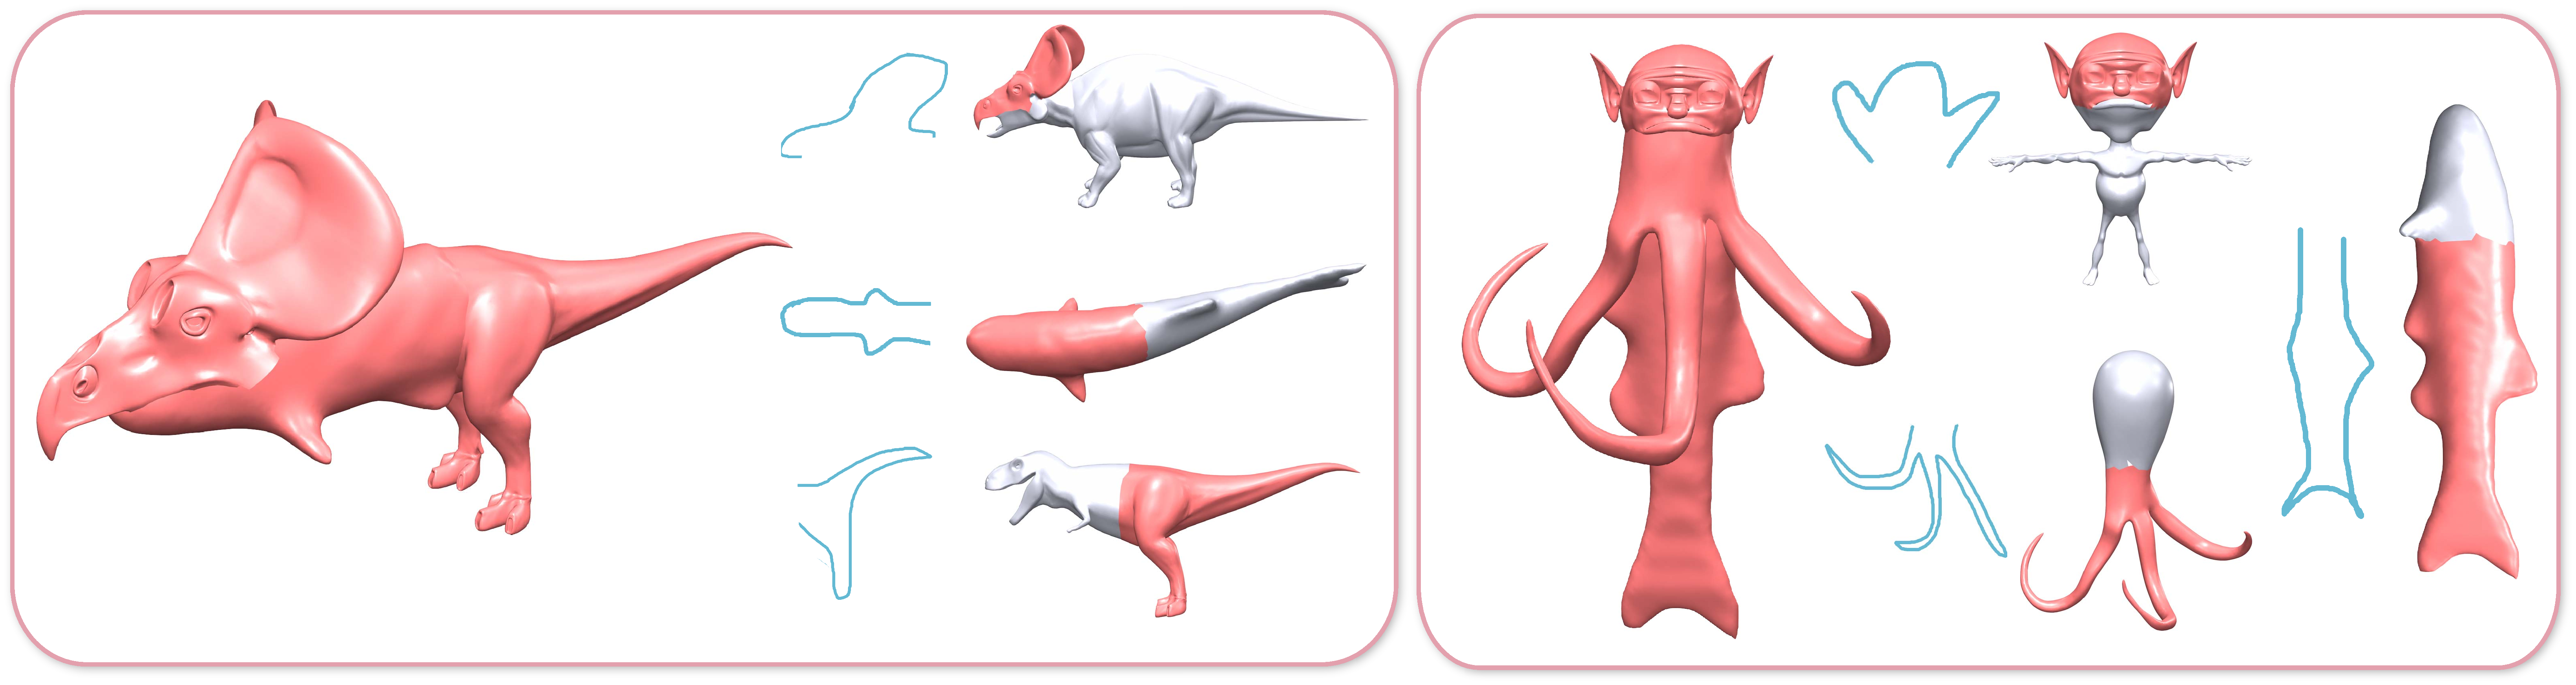
\includegraphics[width=1.05\linewidth]{./Material/CTModels.pdf}
\caption{Examples of sketch-driven assembly-based modeling. In each subfigure, we show the designed models (red), the user's sketches (blue), and the part suggestions selected by the user.}\label{fig:CTModels}
\end{figure}

\begin{figure}\centering
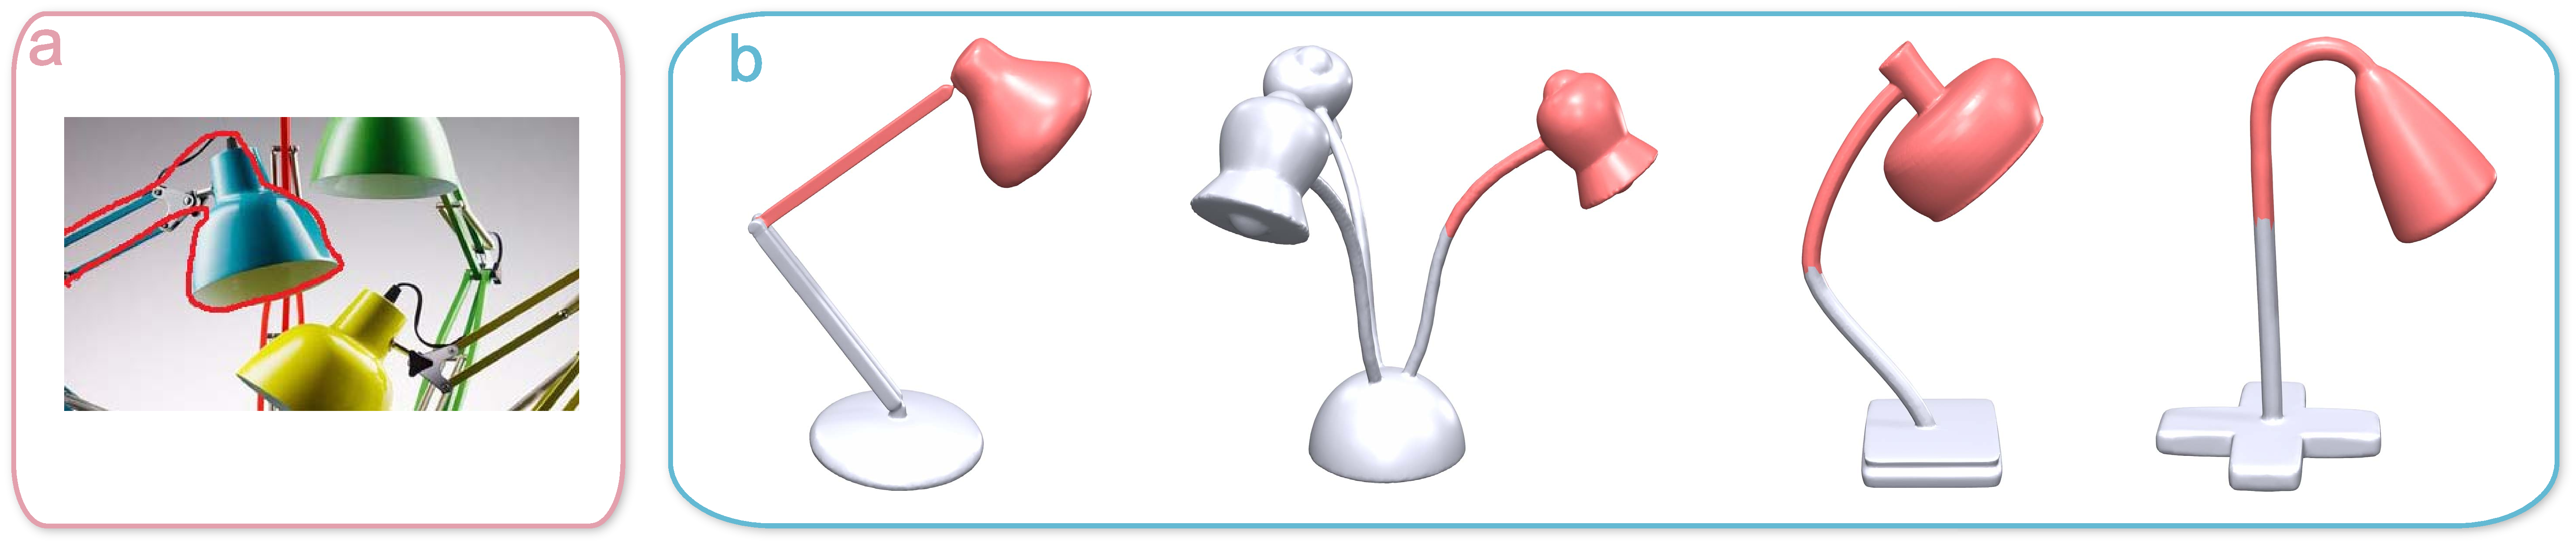
\includegraphics[width=1.05\linewidth]{./Material/Sketch2Scene.pdf}
\caption{Example of contour-driven shape completion. Given a photograph of an occluded lamp, the user traces the outer boundary of the visible portion. This trace is used as the query contour. Our algorithm retrieves possible completions for the object from a database of lamps. (Photo: Xavier Young)}\label{fig:Sketch2Scene}
\end{figure}

\paragraph*{Contour-driven shape completion.} Our algorithm can be used to suggest possible completions for occluded objects in images, an important application in computer vision and image editing. Given a photograph with an occluded object, we manually or automatically trace the boundary of the visible portion and use this trace as input to our algorithm, which retrieves possible completions of the shape from the database. Here, 2D-3D partial matching directly helps us infer the occluded portion. The process is illustrated in Figure \ref{fig:Sketch2Scene}. Alternatively, instead of starting with a photo, the user may directly draw a novel sketch with some occluded components, for example when constructing a complex 3D scene by sketching~\cite{KunXu2013}. Here, too, our algorithm can be used to help recover hidden geometry.

\begin{figure}\centering
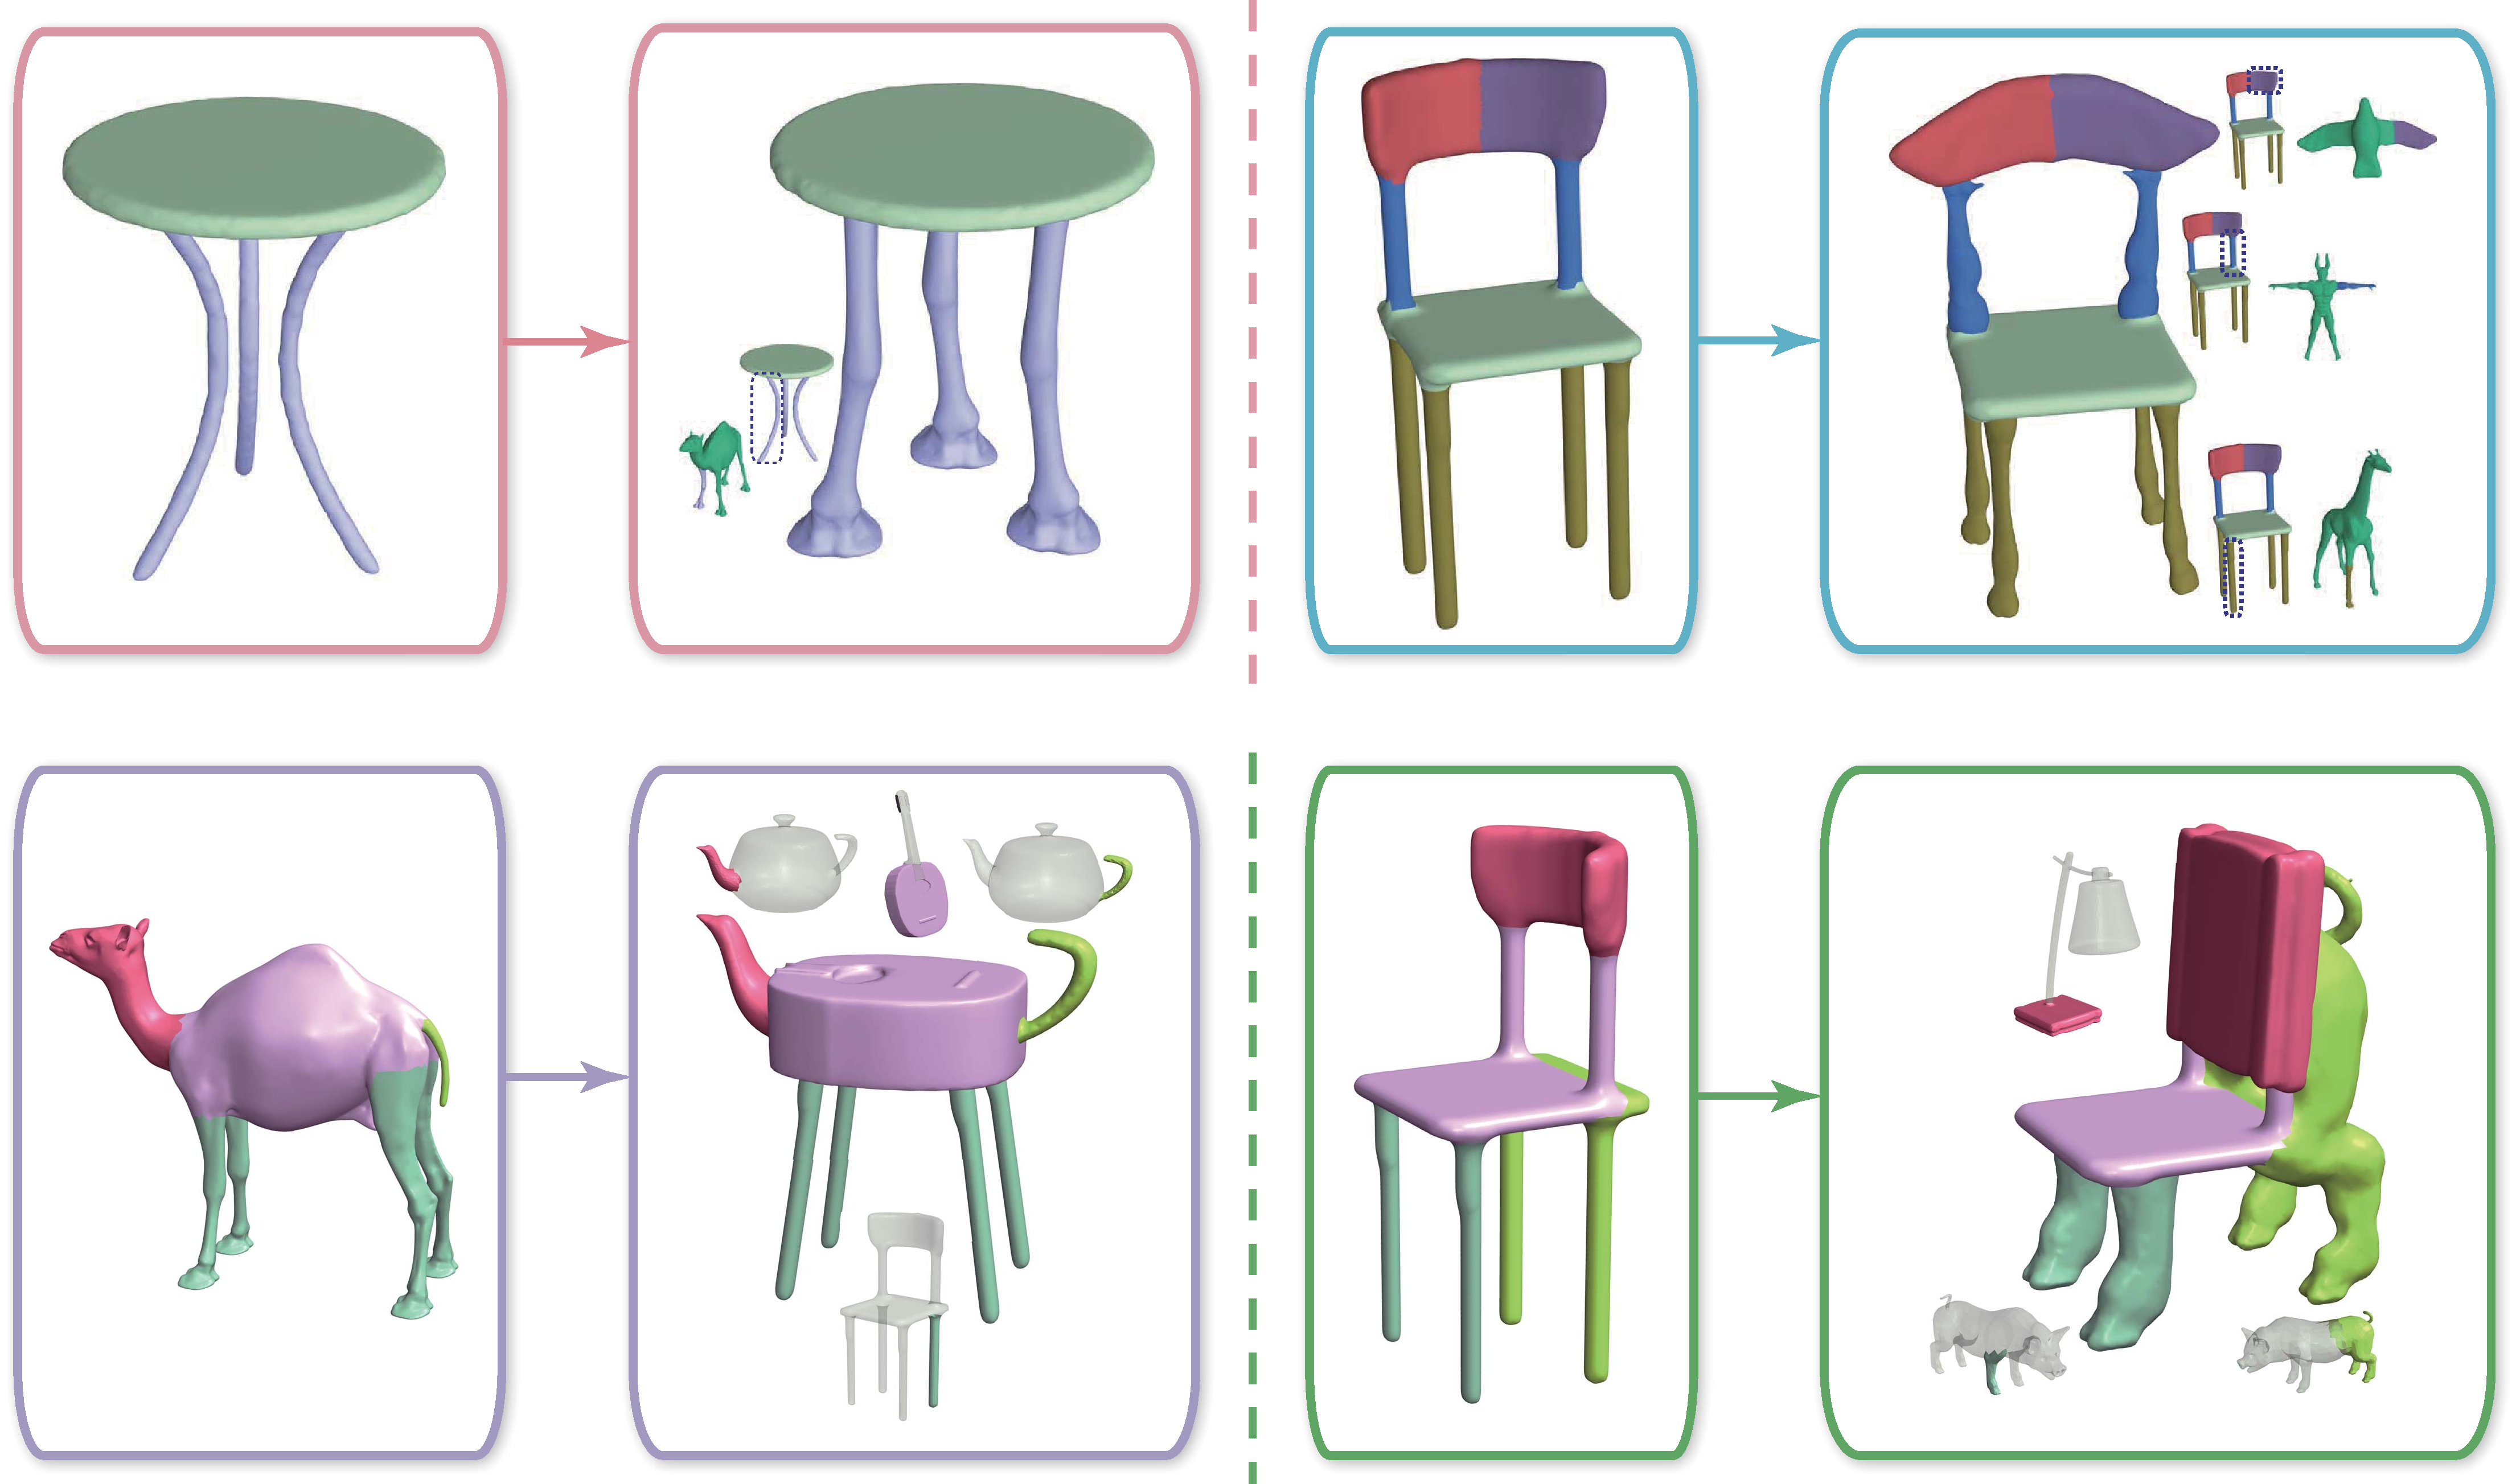
\includegraphics[width=\linewidth]{./Material/ShapeVariation.pdf}
\caption{Examples of shape variations created with our method. Given a segmented model (left), we can use one part as the query to retrieve similar parts from the database. The selected retrieved part is composited with the non-query parts to create a new shape (right) with the same layout as the original shape.}\label{fig:SegedAsInput}
\end{figure}

\paragraph*{Photo-driven part-based modeling.} \hl{Our algorithm can be used to assemble the 3D shape in images. Given a photo with an object, the use draw sketches by tracing the contour of the parts of the shape in the photo. our method retrieves candidate parts from the database according to the user's sketch. The user selects the appropriate parts and assemble the 3D shape in the photo. Figure } \ref{fig:PhotoModeling}\hl{ shows an example.}

\begin{figure}\centering
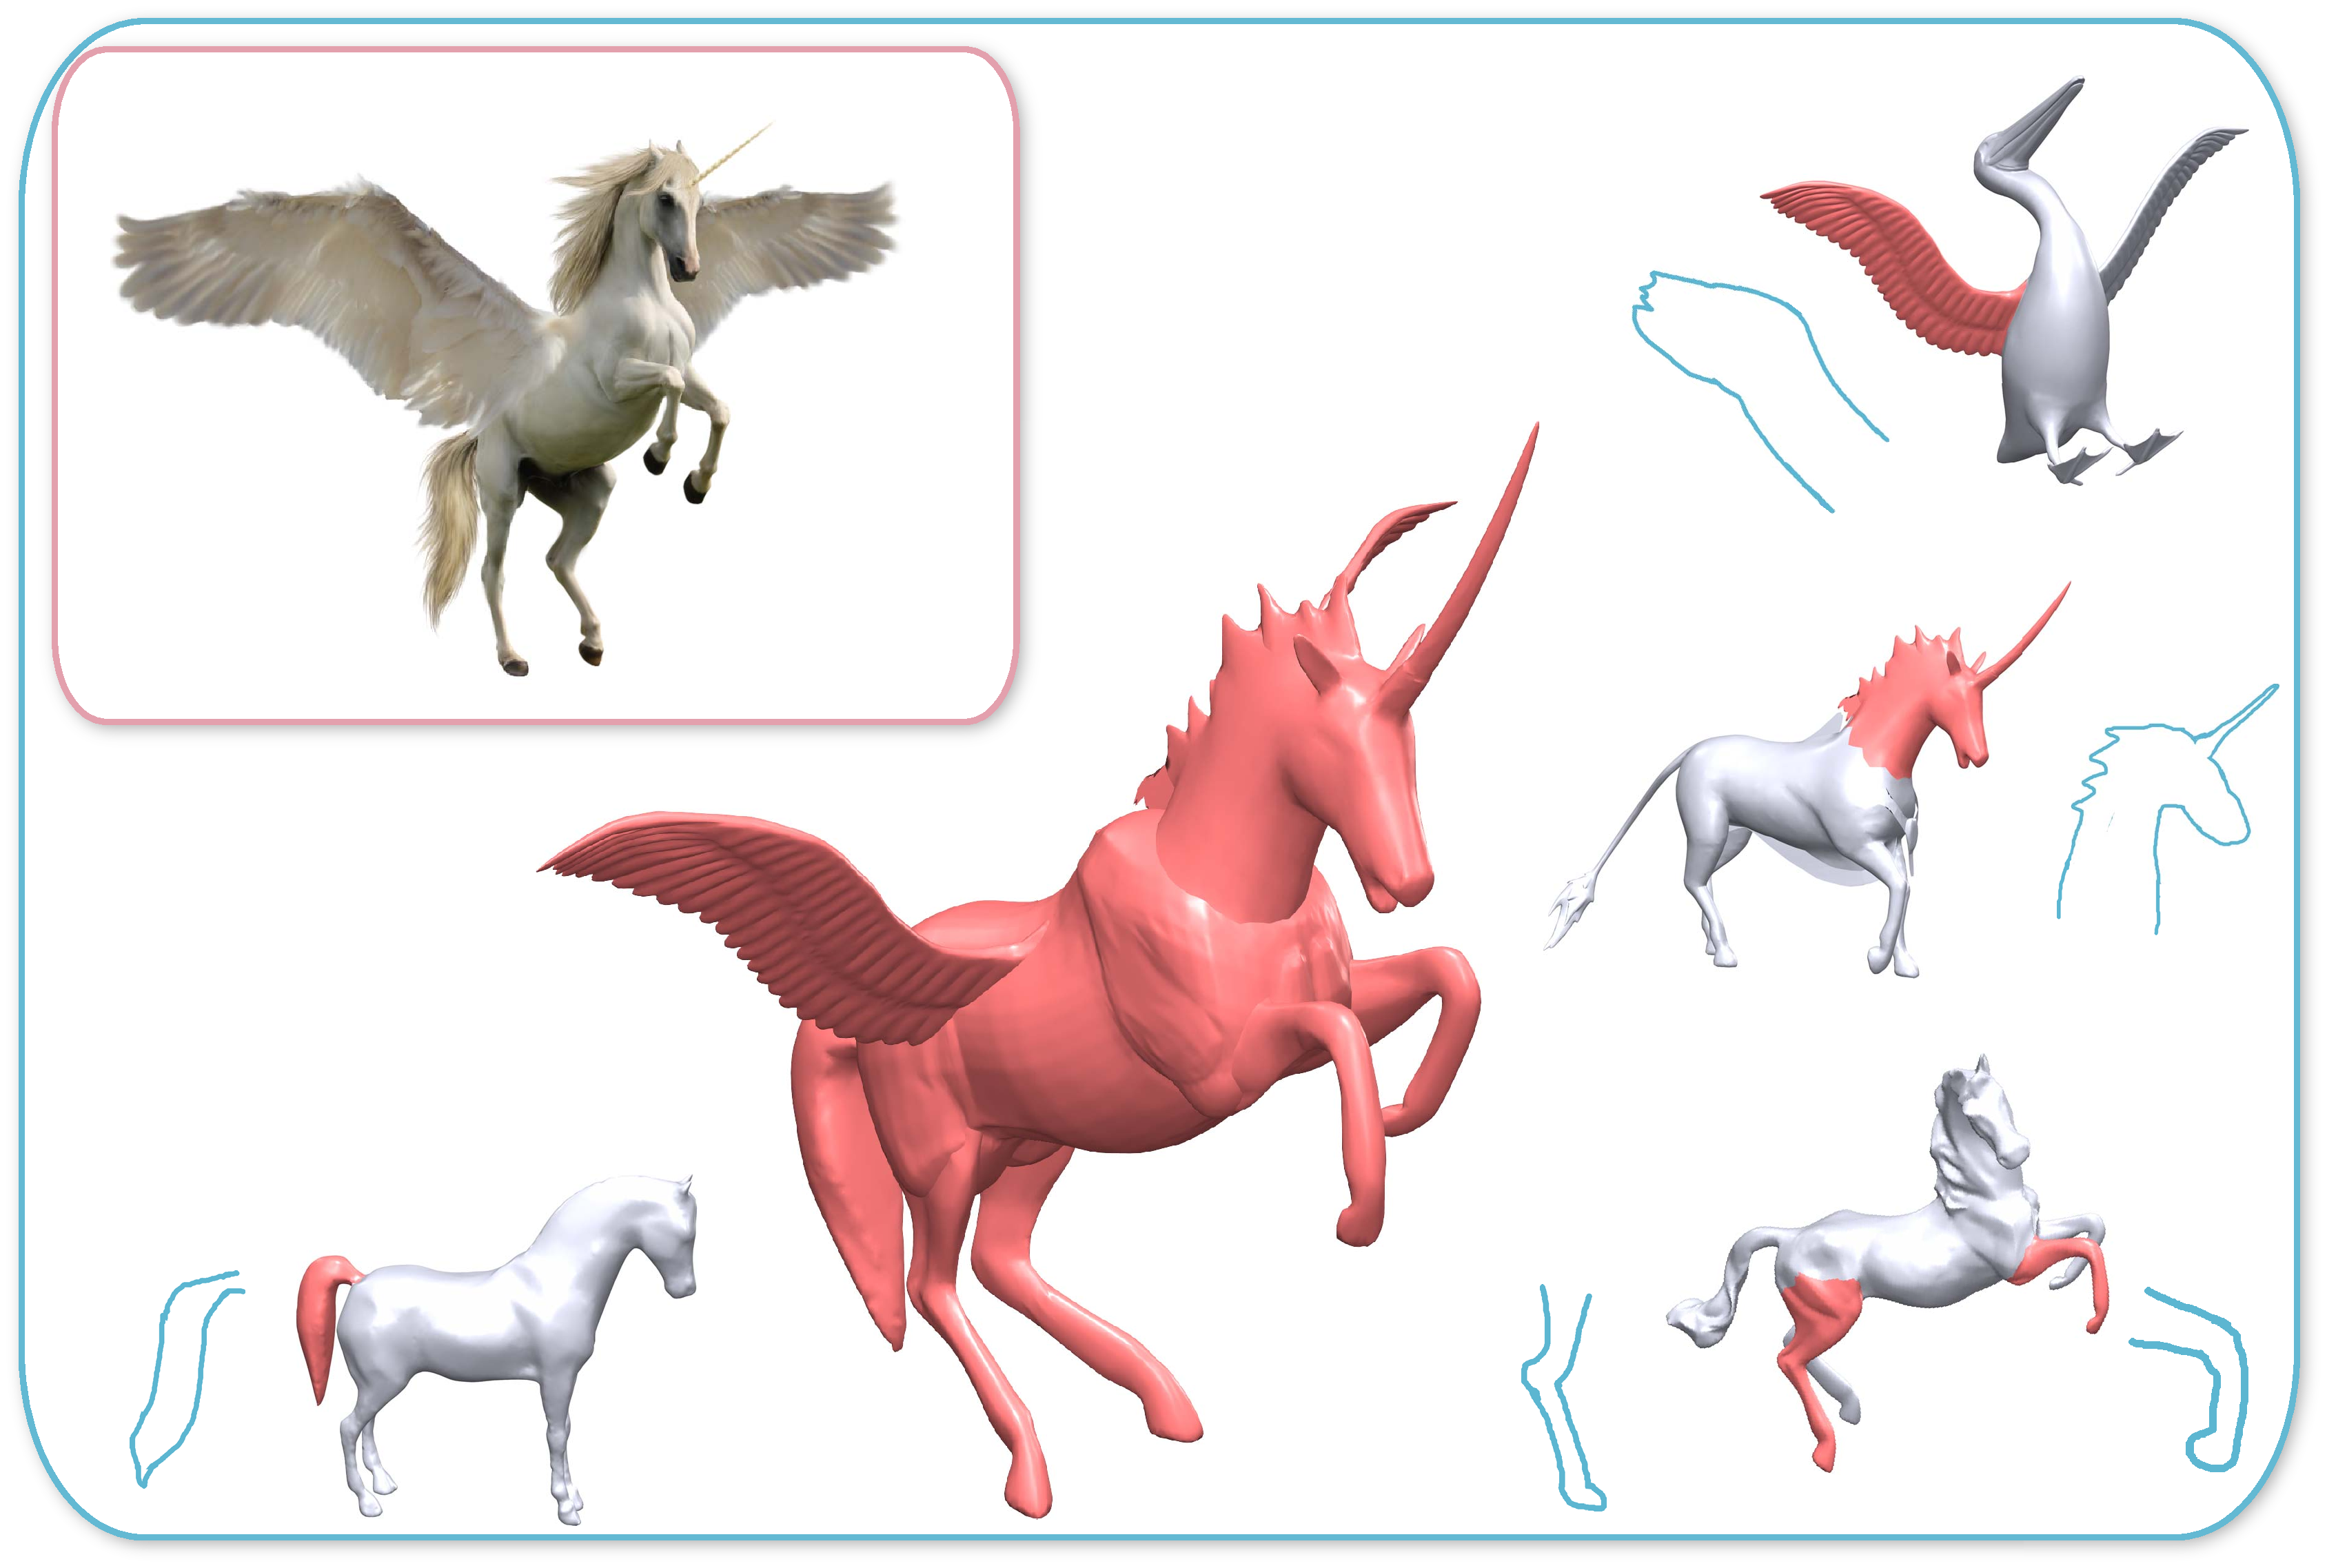
\includegraphics[width=\linewidth]{./Material/PhotoDrivenModeling.pdf}
\caption{Example of photo-driven part-based modeling. Given the photo (on the top left corner), the user sketches the contour of the parts of the shape. Our method extract parts from the database. The user selects the parts and assemble the 3D shape (middle) in the photo.}\label{fig:SegedAsInput}
\end{figure}

\paragraph*{Shape variation.} Our pipeline can be used to generate shape variations by simple adaption, as shown in Figure \ref{fig:SegedAsInput}. Given a segmented shape, we can use any part of the shape as a query to retrieve similar parts from the shape database. The chosen retrieved part can then be used to replace the original part to create shape variations. To extract a query contour from the source part, to be used as the 2D search key in our algorithm, we first perform Principal Component Analysis (PCA) on the part. Then, we take the view perpendicular to the plane containing the first and second principal directions of the part to calculate the query contour.

\begin{figure}\centering
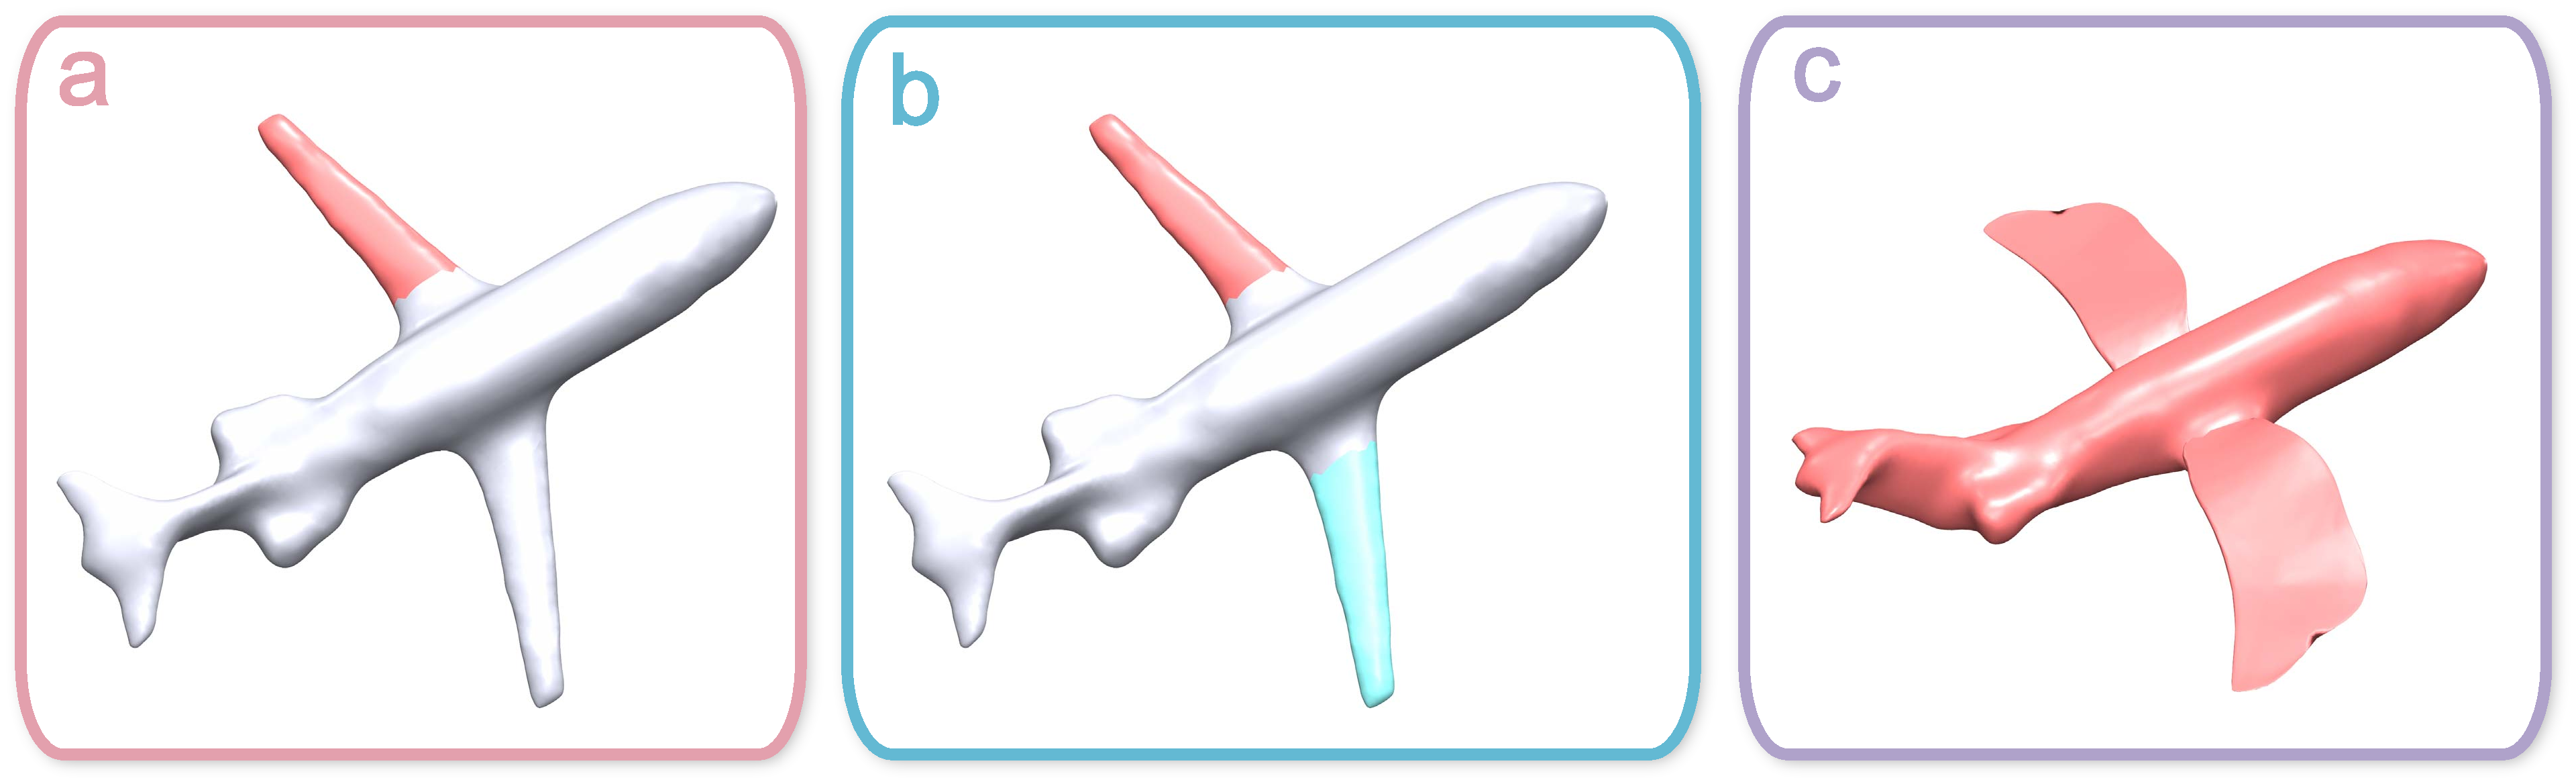
\includegraphics[width=1.0\linewidth]{./Material/SymSel.pdf}
\caption{Example of symmetry-aware selection and editing. The user selects an arbitrary region of a shape (a). Note that the region is not the complete wing, i.e. it is not a ``standard'' segment. We use our algorithm as a fast partial matching technique, to find other parts in the same shape with the same contour. This yields the corresponding region of the other wing as a symmetric counterpart (b). Finally, the symmetric pair may be replaced by another, retrieved from a database using our ``shape variations'' approach (c).}\label{fig:SymSel}
\end{figure}

\paragraph*{Symmetry-aware selection and editing.} Our method can also be used to select a group of similar elements in a single shape for further editing. For example, in Fig \ref{fig:SymSel}, the user picks an arbitrary region of the leg of a table. The corresponding regions of the other legs will be automatically identified, by partial matching of the contour of the selected region with the rest of the shape itself. Subsequently, the entire selected group can be replaced by similar parts retrieved from the database, as in the ``shape variations'' applicaton.

\paragraph*{Part suggestion.} Our on-the-fly part extraction technique can be used to suggest parts to extend a base shape~\cite{datadrivenvladenaisa2010,probabilisticreasoningvladlensg2011}. In contrast to previous methods, we do not require a pre-segmented database. Given a query shape, we treat its outline as the query contour and feed it to the algorithm. Our method matches the contour to parts of exemplar shapes, and suggests maximal connected components of the {\em rest} of the exemplar as suggestions for creatively extending the shape. The suggested parts can be irregular ones or from different shape families (see Figure \ref{fig:appl}).

\begin{figure}[t]\centering
\includegraphics[width=1.05\linewidth]{./Material/Appl.pdf}
\caption{Examples of part suggestions. Given the query shapes (in green), our system presents a list of part suggestions (in purple). The assembled shapes are shown below the suggested parts.}\label{fig:appl}
\end{figure}

\paragraph*{Multi-scale part suggestion.} Our system can suggest parts at various scales. Given a part \st{suggested} \hl{retrieved} by the method above, we perform normalized cuts~\cite{randomizedcutsfunkhousertog2008} on \hl{the SFG corresponding to the retrieved part} \st{its corresponding sub-SFG} to generate $T_n$ segments, each of which consists of a group of adjacent super-faces. $T_n$ is defined as:
\[{T_n} = \frac{{w(Vol(P_M)-Vol\left( {{p_p})} \right)}}{{Vol\left( {{p_p}} \right)}},\] where $Vol\left( \cdot \right)$ is the volume of an object, $P_M$ is the retrieved database model, $p_p$ is the part in the database model corresponding to the query \hl{(corresponding part)}, and the weight $w = 2$. We constrain $T_n$ to lie between 1 and 7. We rank the segments in ascending order by their distance to the corresponding part. \hl{The distance is defined as the Euclidean distance between the OBB of the segment and the corresponding part. Now, given a scale $S$, we can suggest the segments with this scale (the segments whose distance to the corresponding part is less than or equal to $S$)}. An example is given in Figure \ref{fig:MSPS}.

\begin{figure}[t]\centering
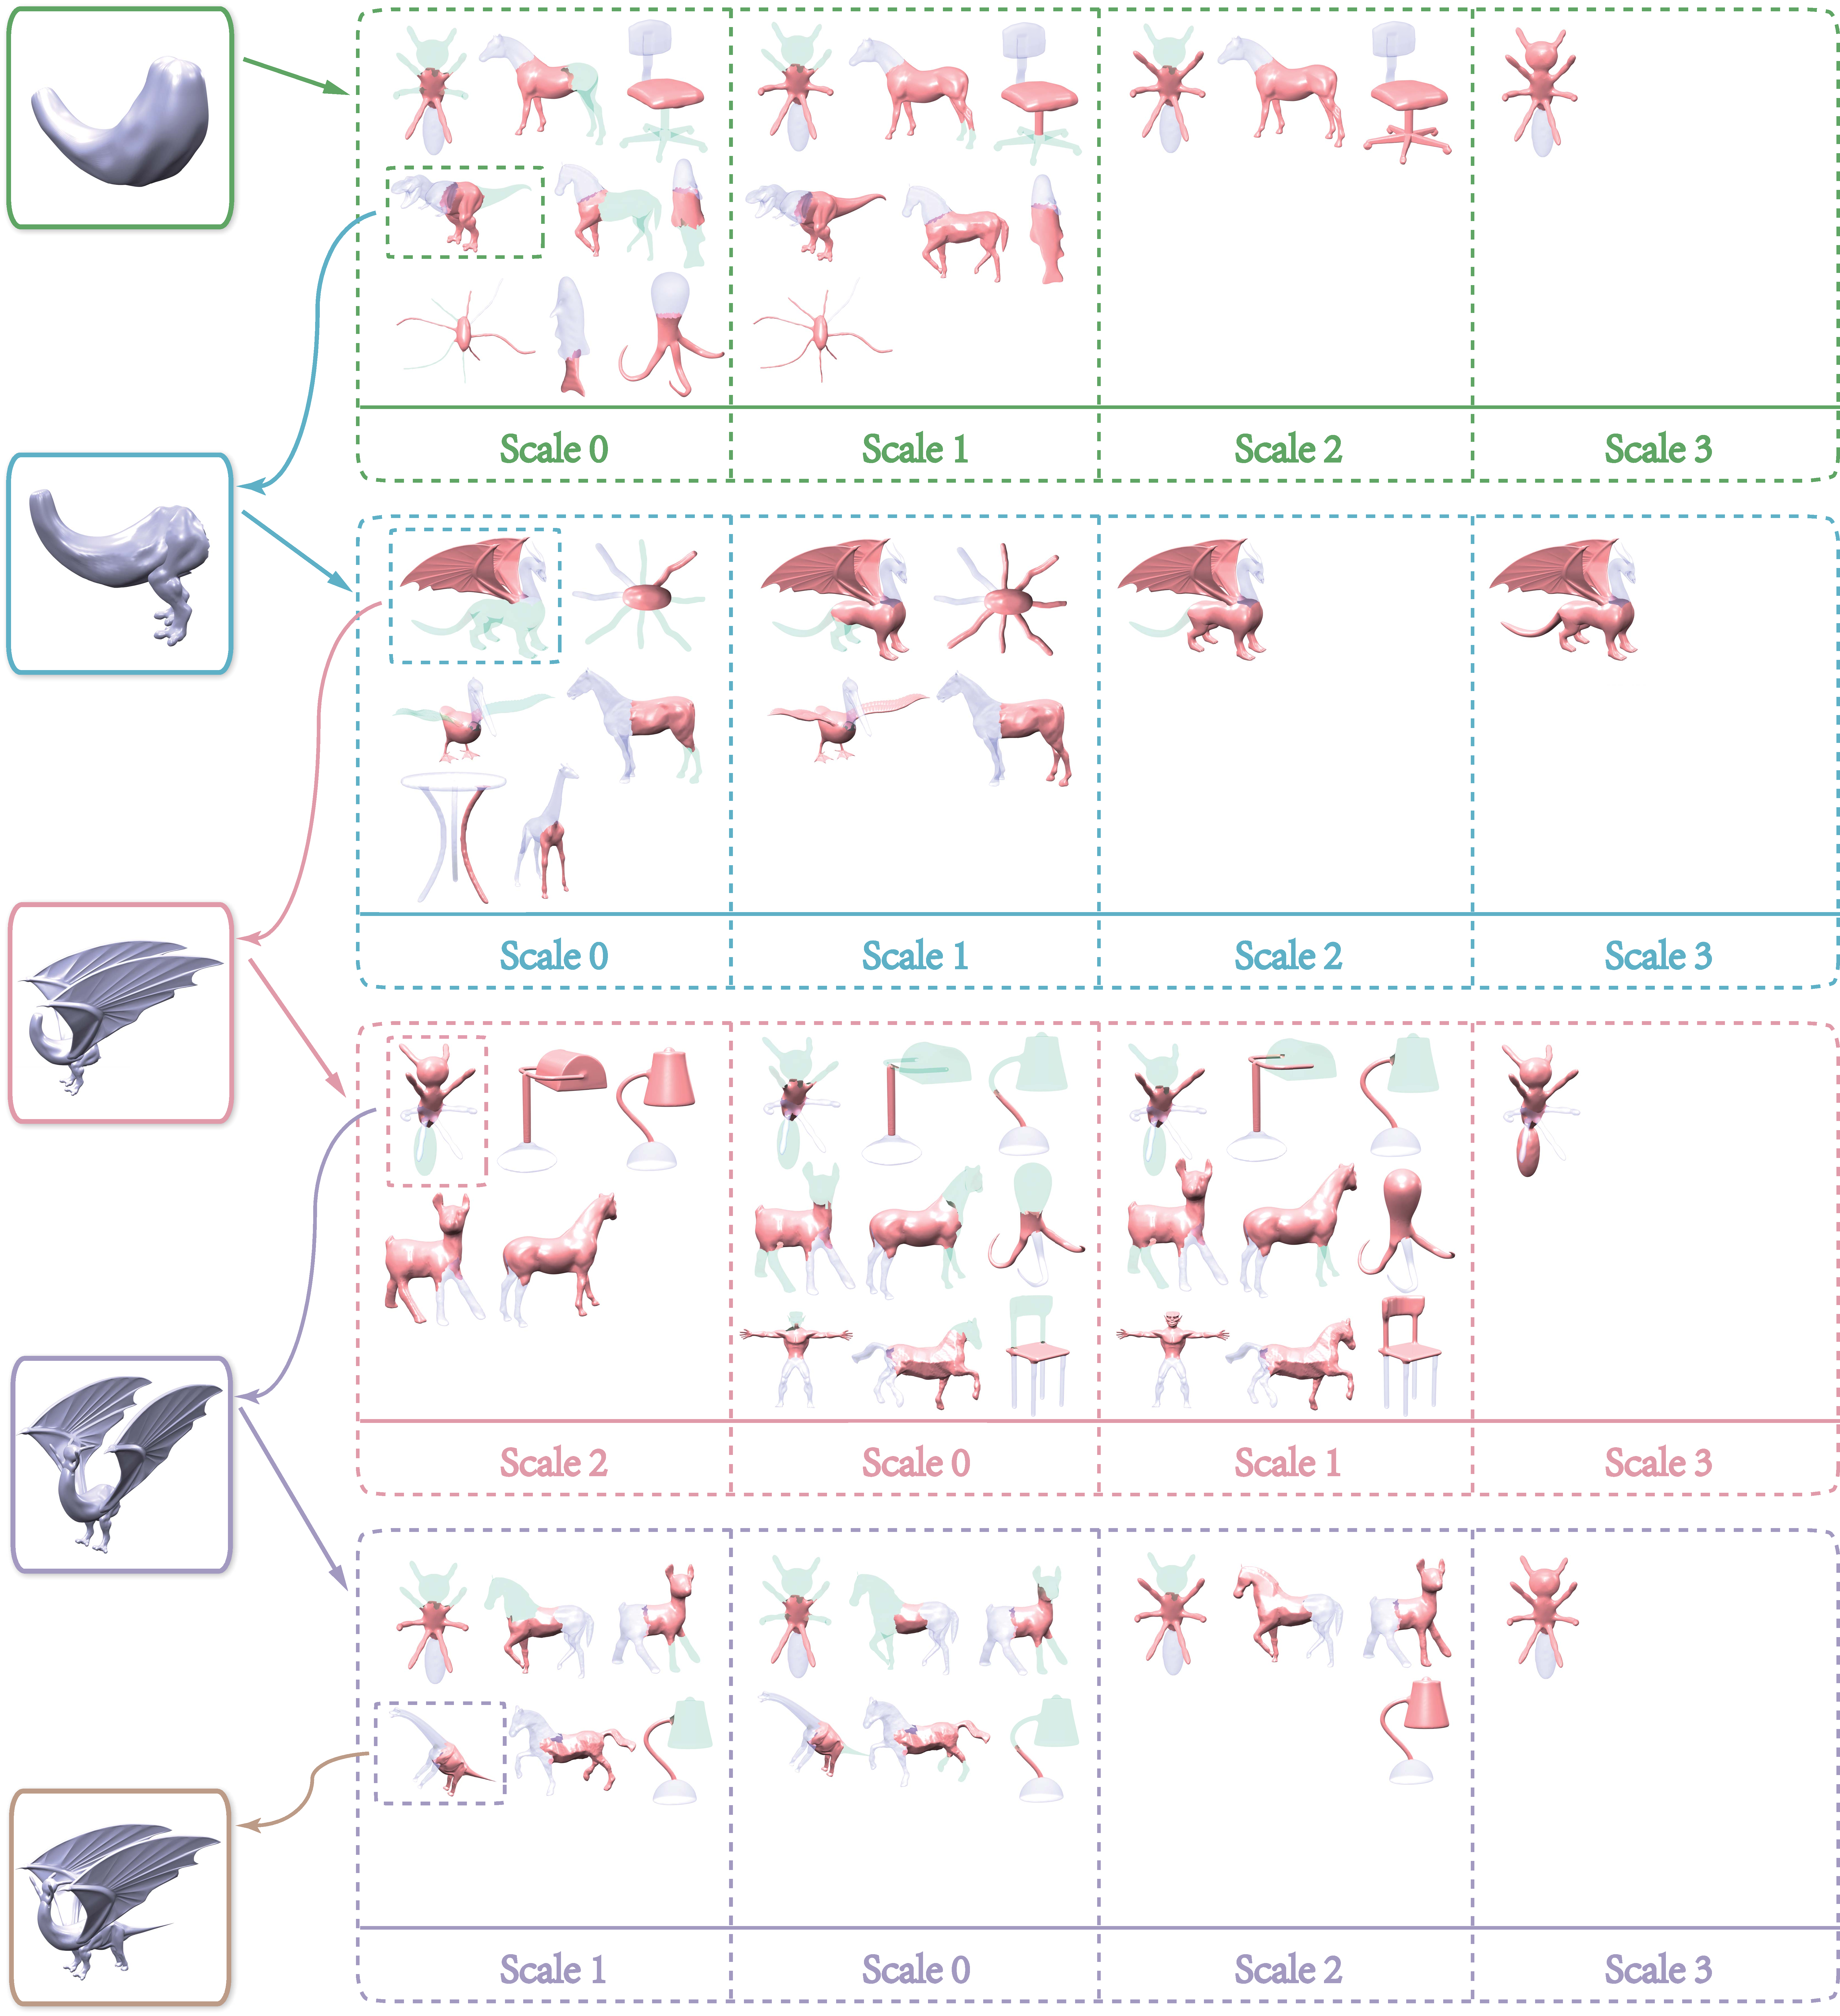
\includegraphics[width=1.05\linewidth]{./Material/MSPS.pdf}
\caption{An example of multi-scale part suggestion. The initial shape and subsequent working models, used as queries, are listed in the left column. On the right, we show the suggested parts (red) at different scales for each modeling step. The parts corresponding to the queries are marked in light blue. The other parts are marked in light green.}\label{fig:MSPS}
\end{figure}



%%%%%%%%%%%%%%%%%%%%%%%%%%%%%%%%%%%%%%%%%%%%%%%%%%%%%%%%%%%%%%%%%%%%%%%%%%%%%%%%%%%%%%%%%%%%%%%%%%%%%%%%%%%%
\section{Evaluation}

We have validated our prototype system, written in C++, on a 64-bit desktop machine with a 3.5 GHz Intel Core I7-3770K processor, 8GB memory, and an Nvidia GeForce GTX 660 GPU video card. \hl{Figure }\ref{fig:MoreRetrievalRes}\hl{ shows retrieval results with the user sketch.}

\begin{figure}\centering
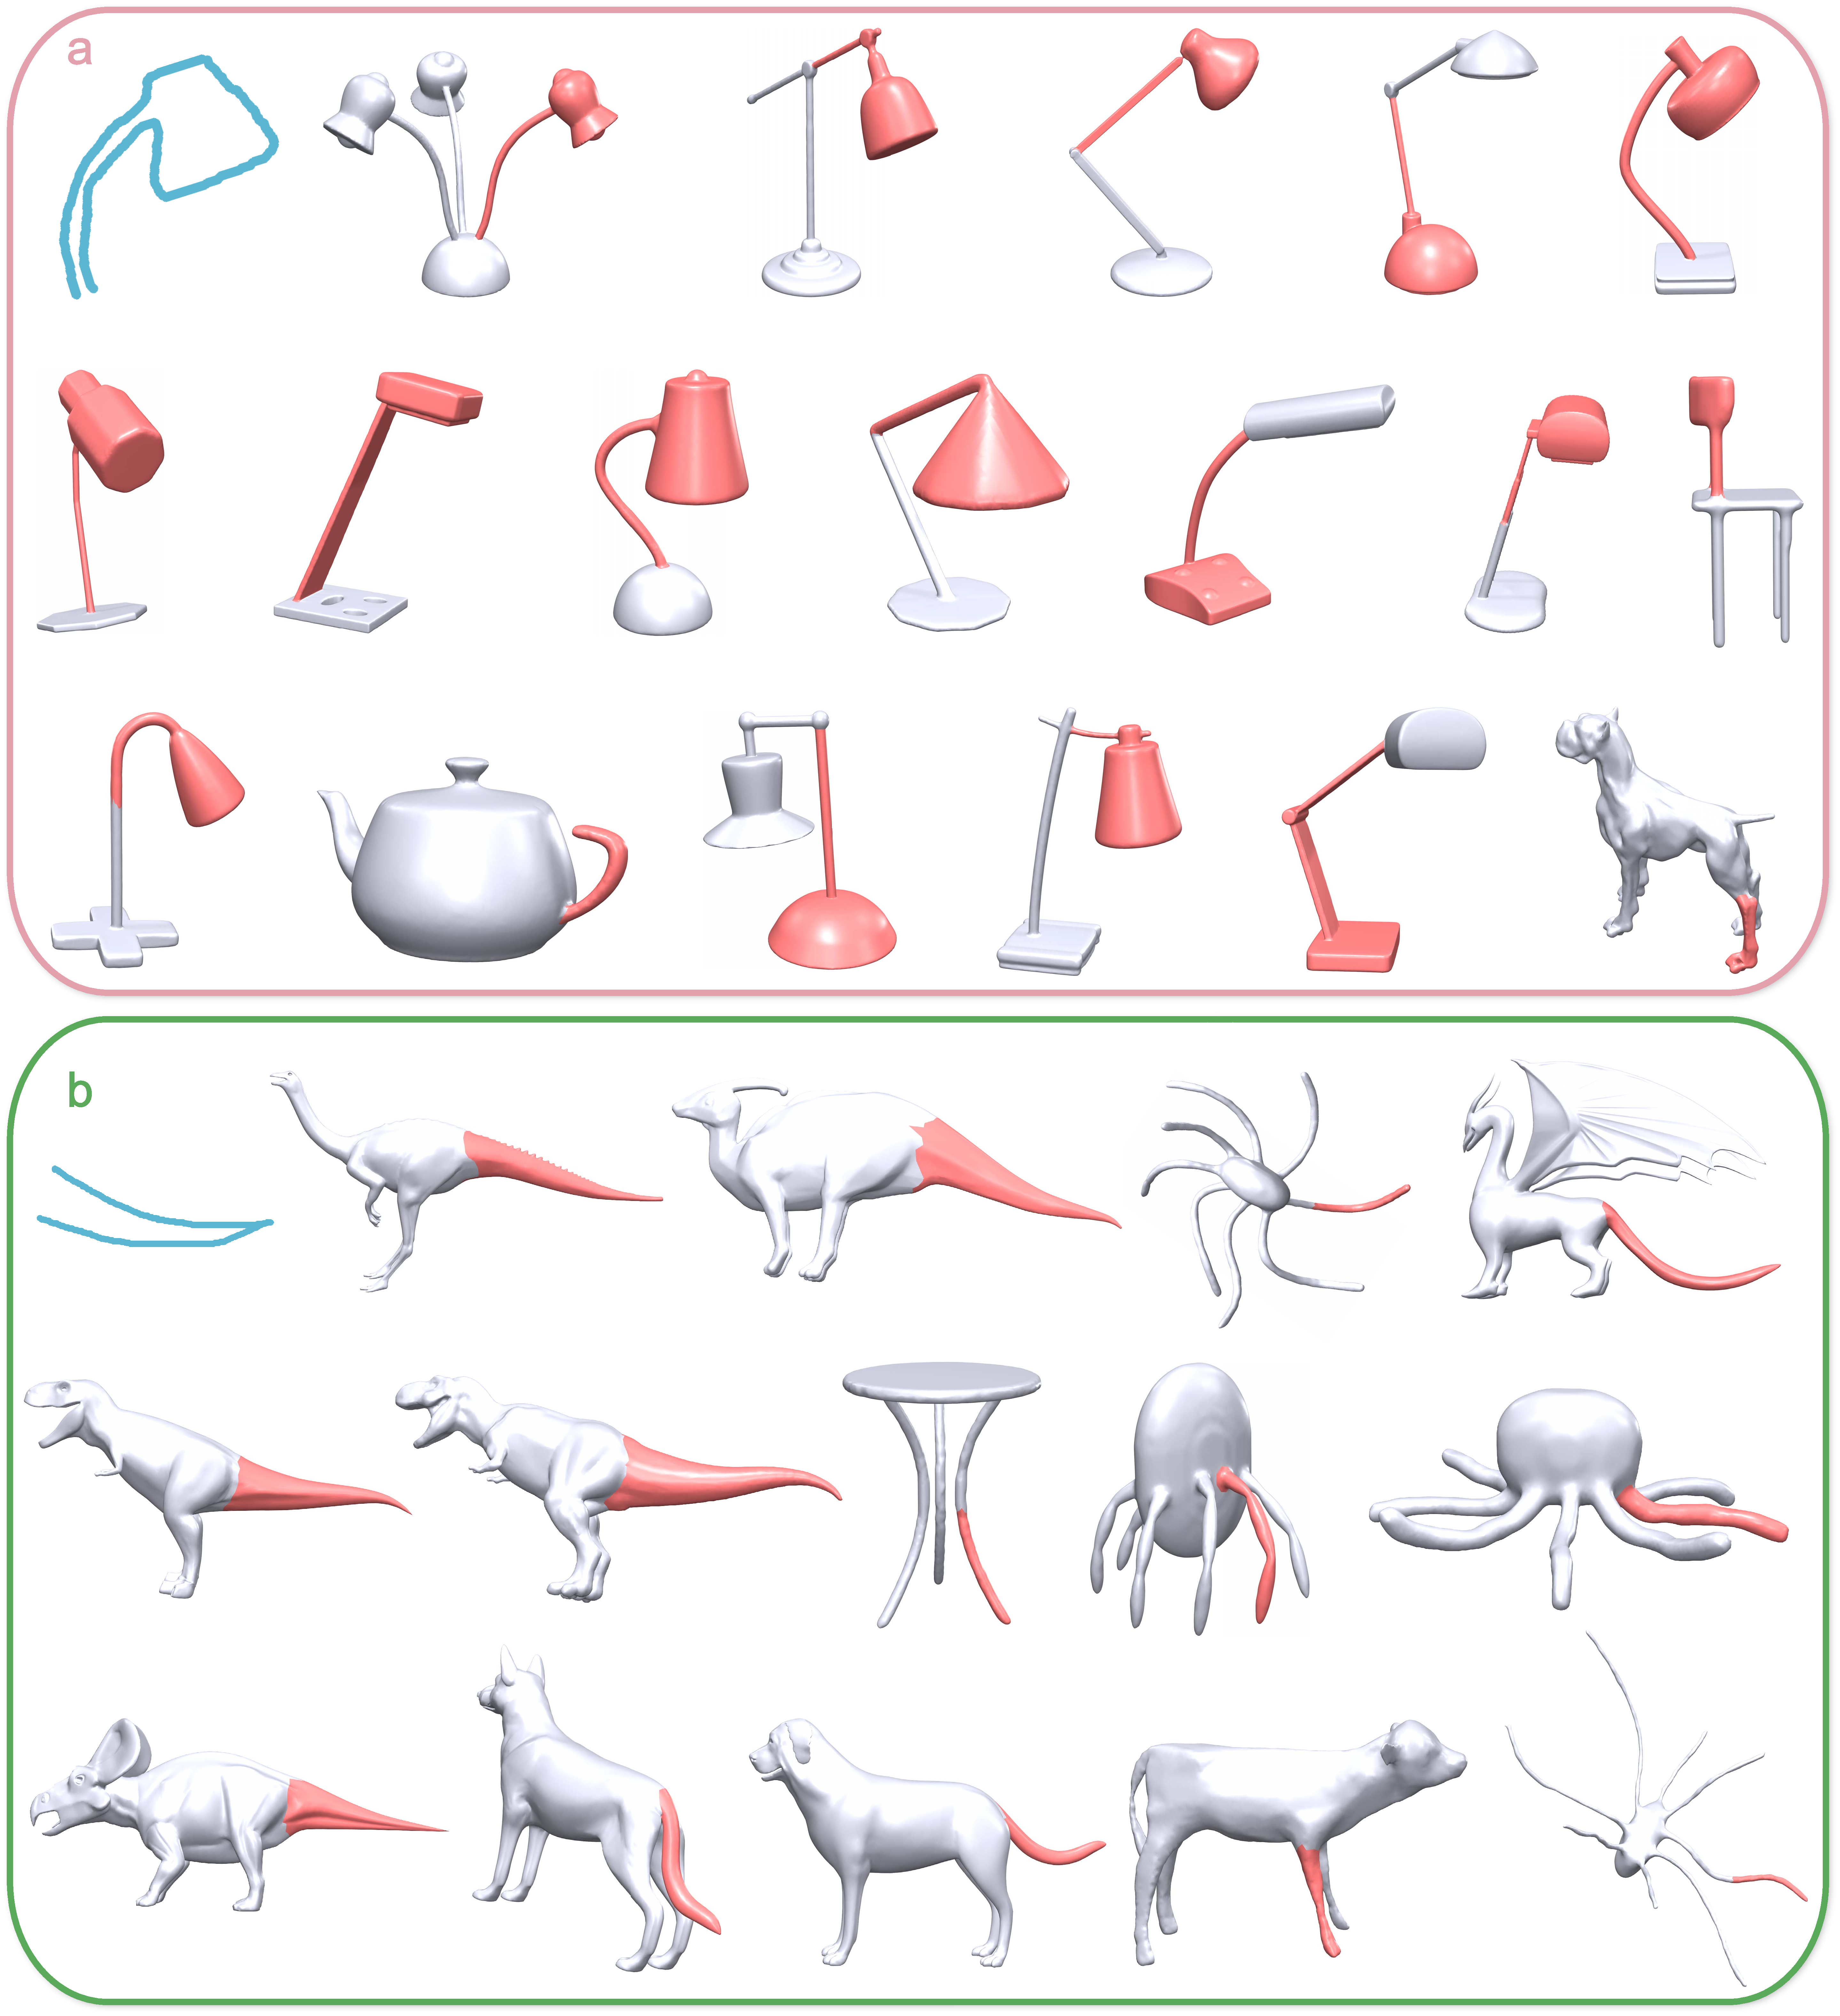
\includegraphics[width=1.05\linewidth]{./Material/MoreRetrievalRes.pdf}
\caption{Retrieval results generated with our method. The retrieved parts are ranked from left to right, form top to bottom.}\label{fig:MoreRetrievalRes}
\end{figure}

There are 513 3D shapes in our database. From these shapes, we extracted 10,773 contours. It took $\sim$3.5 hours to organize these contours into an {\RCKNNG}. The average time to construct the super-face graph of a shape is 20 seconds. Because of the super-face graph representation, our part extraction is real-time. The time for the coarse and fine level extractions for one model is 0.15ms and 10.3ms on average, respectively. Thanks to the two acceleration structures ({\RCKNNG} and SFG) and the coarse-to-fine part extraction strategy, our system can run interactively during the design process. Once a user finishes drawing the sketch, it takes 0.56-0.61 seconds (with GPU and multi-core acceleration) on average for our system to present part suggestions.

\paragraph*{{\RCKNNG} Retrieval Performance.} To evaluate the performance of our {\RCKNNG}, we compare the following methods:
\begin{enumerate}
\setlength{\itemsep}{3pt}
\setlength{\parskip}{0pt}
\setlength{\parsep}{0pt}
\item Traditional (single-layer) $k$NNG constructed by brute force.
\item Wang's randomized $k$NNG approximation~\cite{scalableknnjingwangcvpr2012}.
\item {\RCKNNG} constructed by brute force.
\item {\RCKNNG} with Wang's randomized approximation (\mbox{\textbf{our method}}).
\end{enumerate}
For the two $k$NN graph methods (1 and 2), nodes of the graph are complete shape contours. Node adjacencies and edge weights are identified by global comparison of shape contours. \hl{To compute the contour descriptor of the shape contour, the shape contour is first sampled under 3 different scales. 50, 150, and 250 points along the contour are sampled respectively. The contour descriptor is calculated for the sampled points.} When searching for partial matches to a query contour, we must extract similar contour sections explicitly, significantly slowing down both methods.

For the two {\RCKNNG} methods (3 and 4), nodes of the graph are contour sections (Section \ref{sec:acc}). In our evaluations, we set $k = 20$  and extract $6$ sections from each shape contour.

The retrieval performance for each method is shown in Table \ref{tab:RCKNNGComp}. It is clear that RC-$k$NNG with Wang's method, as proposed in this paper, has the best performance. For retrieval, it is about 97 times faster than Wang's $k$NNG, with only 3 times the construction time. The $k$NNG approaches, which require explicit partial matching at runtime, are much slower.

\hl{We could clearly see the x improvement from Table }\ref{tab:RCKNNGComp}\hl{. The retrieval results generated by the four methods is shown in figure }\ref{fig:RCKNNGComp}\hl{. For the two $k$NNG methods, the retrieved parts are nearly the same. For the two {\RCKNNG} methods, the retrieved parts are nearly the same. But the retrieved parts are different for the two types of the methods.}
%--------------------------
\begin{table}\centering \renewcommand\arraystretch{1.3}
\begin{tabular}{|c|c|c|c|}
\hline \diagbox{Algorithm}{Performance}       & RT  & CT         & ME  \\
\hline BF $k$NNG                     & 4.54s  & 51.7h   & 0.075   \\
\hline Wang $k$NNG                   & 5.68s  & 1.15h   & 0.0795  \\
\hline BF {\RCKNNG}   & 0.053s & 33.89h & 0.07  \\
\hline Wang {\RCKNNG}            & 0.058s & 3.52h  & 0.07  \\
\hline
\end{tabular}
\caption{Retrieval performance for different methods on our test dataset. RT is the retrieval time for a query contour. CT is the construction time for the {\RCKNNG} data structure. ME is the matching error for the retrieval results.
BF $K$NNG represents the Brute force $k$NNG method. Wang $k$NNG represents the Wang's $k$NNG approximation method.
BF {\RCKNNG} represents the {\RCKNNG} with the brute force method.
Wang {\RCKNNG} represents the {\RCKNNG} with Wang's method.}\label{tab:RCKNNGComp}
\end{table}
%--------------------------
\begin{figure} \centering
\includegraphics[width=1.0\linewidth]{./Material/RCKNNGComp.pdf}
\caption{Retrieved parts generated with different methods: the brute force $k$NNG method (a), the Wang's randomized $k$NNG approximation method (b),
the {\RCKNNG} with the brute force method (c), and the {\RCKNNG} with Wang's method (d).}
\label{fig:RCKNNGComp}
\end{figure}
%--------------------------
\begin{figure}\centering
\subfigure[Different methods]{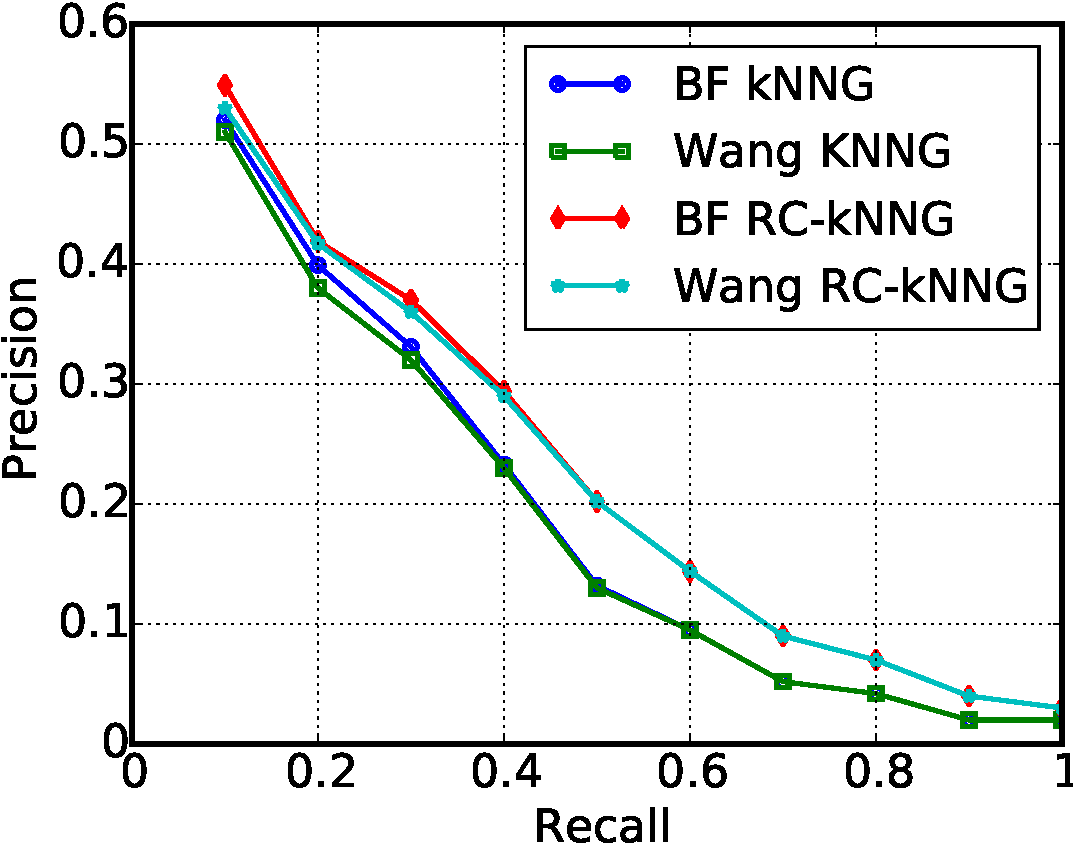
\includegraphics[width=0.49\linewidth]{./Material/PreRecDifAlg.pdf}}
\subfigure[Different camera views]{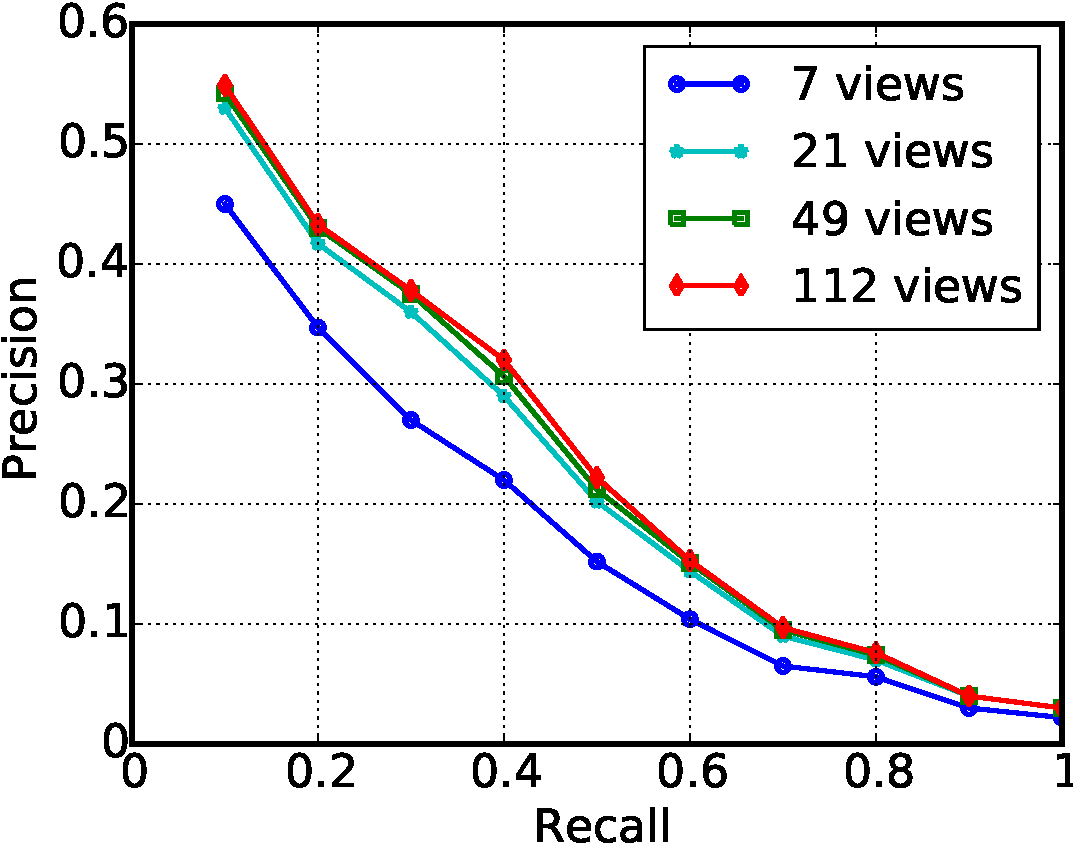
\includegraphics[width=0.49\linewidth]{./Material/PreRecDifViews.pdf}}
\caption{Averaged precision recall curves. (a) compares different retrieval methods. (b) compares different camera views. 
In (a), BF kNNG represents the Brute force $k$NNG method; Wang kNNG represents the Wang's $k$NNG approximation method; 
BF RC-kNNG represents represents the {\RCKNNG} with the brute force method; 
Wang RC-kNNG represents the {\RCKNNG} with Wang's method.}\label{fig:PreRecCurve}
\end{figure}

%--------------------------
\begin{table}\centering \renewcommand\arraystretch{1.3}
\begin{tabular}{|c|c|c|c|}
\hline \diagbox{Step}{SF Count} & 50    & 100    & 200    \\
\hline Construction of SFG      & 20s    & 14.01s  & 19.07s  \\
\hline Coarse extraction (per shape)  & 0.15ms  & 0.77ms   & 3.91ms   \\
\hline Full part extraction    & 560ms  & 577ms  & 605ms  \\
\hline
\end{tabular}
\caption{Timing statistics with different super-face counts. Full part extraction measures the time from launch of a query to generation of a final part.}\label{tab:SFCounts}
\end{table}
%--------------------------

%--------------------------
\begin{table}\centering \renewcommand\arraystretch{1.3}
\begin{tabular}{|c|c|c|c|}
\hline \diagbox{}{SF Count} & 50    & 100    & 200    \\
\hline Matching error      & 0.45     & 0.29   & 0.07   \\
\hline
\end{tabular}
\caption{Matching error statistics with different super-face counts, averaged over a set of 20 test sketches.}\label{tab:MatchError}
\end{table}
%--------------------------

\paragraph*{Increasing Super-Face Counts.} In Table \ref{tab:SFCounts}, we show the timing statistics for different super-face counts. The coarse-level part extraction time is strongly dependent on the number of super-faces. However, this is a relatively fast step so this dependence does not significantly hurt overall performance. Overall, despite quadrupling the number of super-faces, part extraction remains interactive, completing in well under 1s.

In Figure \ref{fig:SFCountsPartQuality}, we show the qualitative improvement in part extraction as we increase the number of super-faces. With fewer super-faces, the search space is relatively coarse and the extracted parts need not perfectly match the sketch. As we increase the number of super-faces, the search space becomes more fine-grained. The part contours match the sketch better and better, and the part boundaries are less constrained to follow suboptimal cuts. We quantitatively evaluate the quality of the extracted part by comparing the contour of the extracted part with the user's sketch in terms of the contour descriptor introduced in Section \ref{subsec:CtourDesc}. Table \ref{tab:MatchError} shows the matching error statistics for different super-face counts. Note that the error decreases substantially as the shape representation becomes more fine-grained.

\begin{figure}[h!] \centering
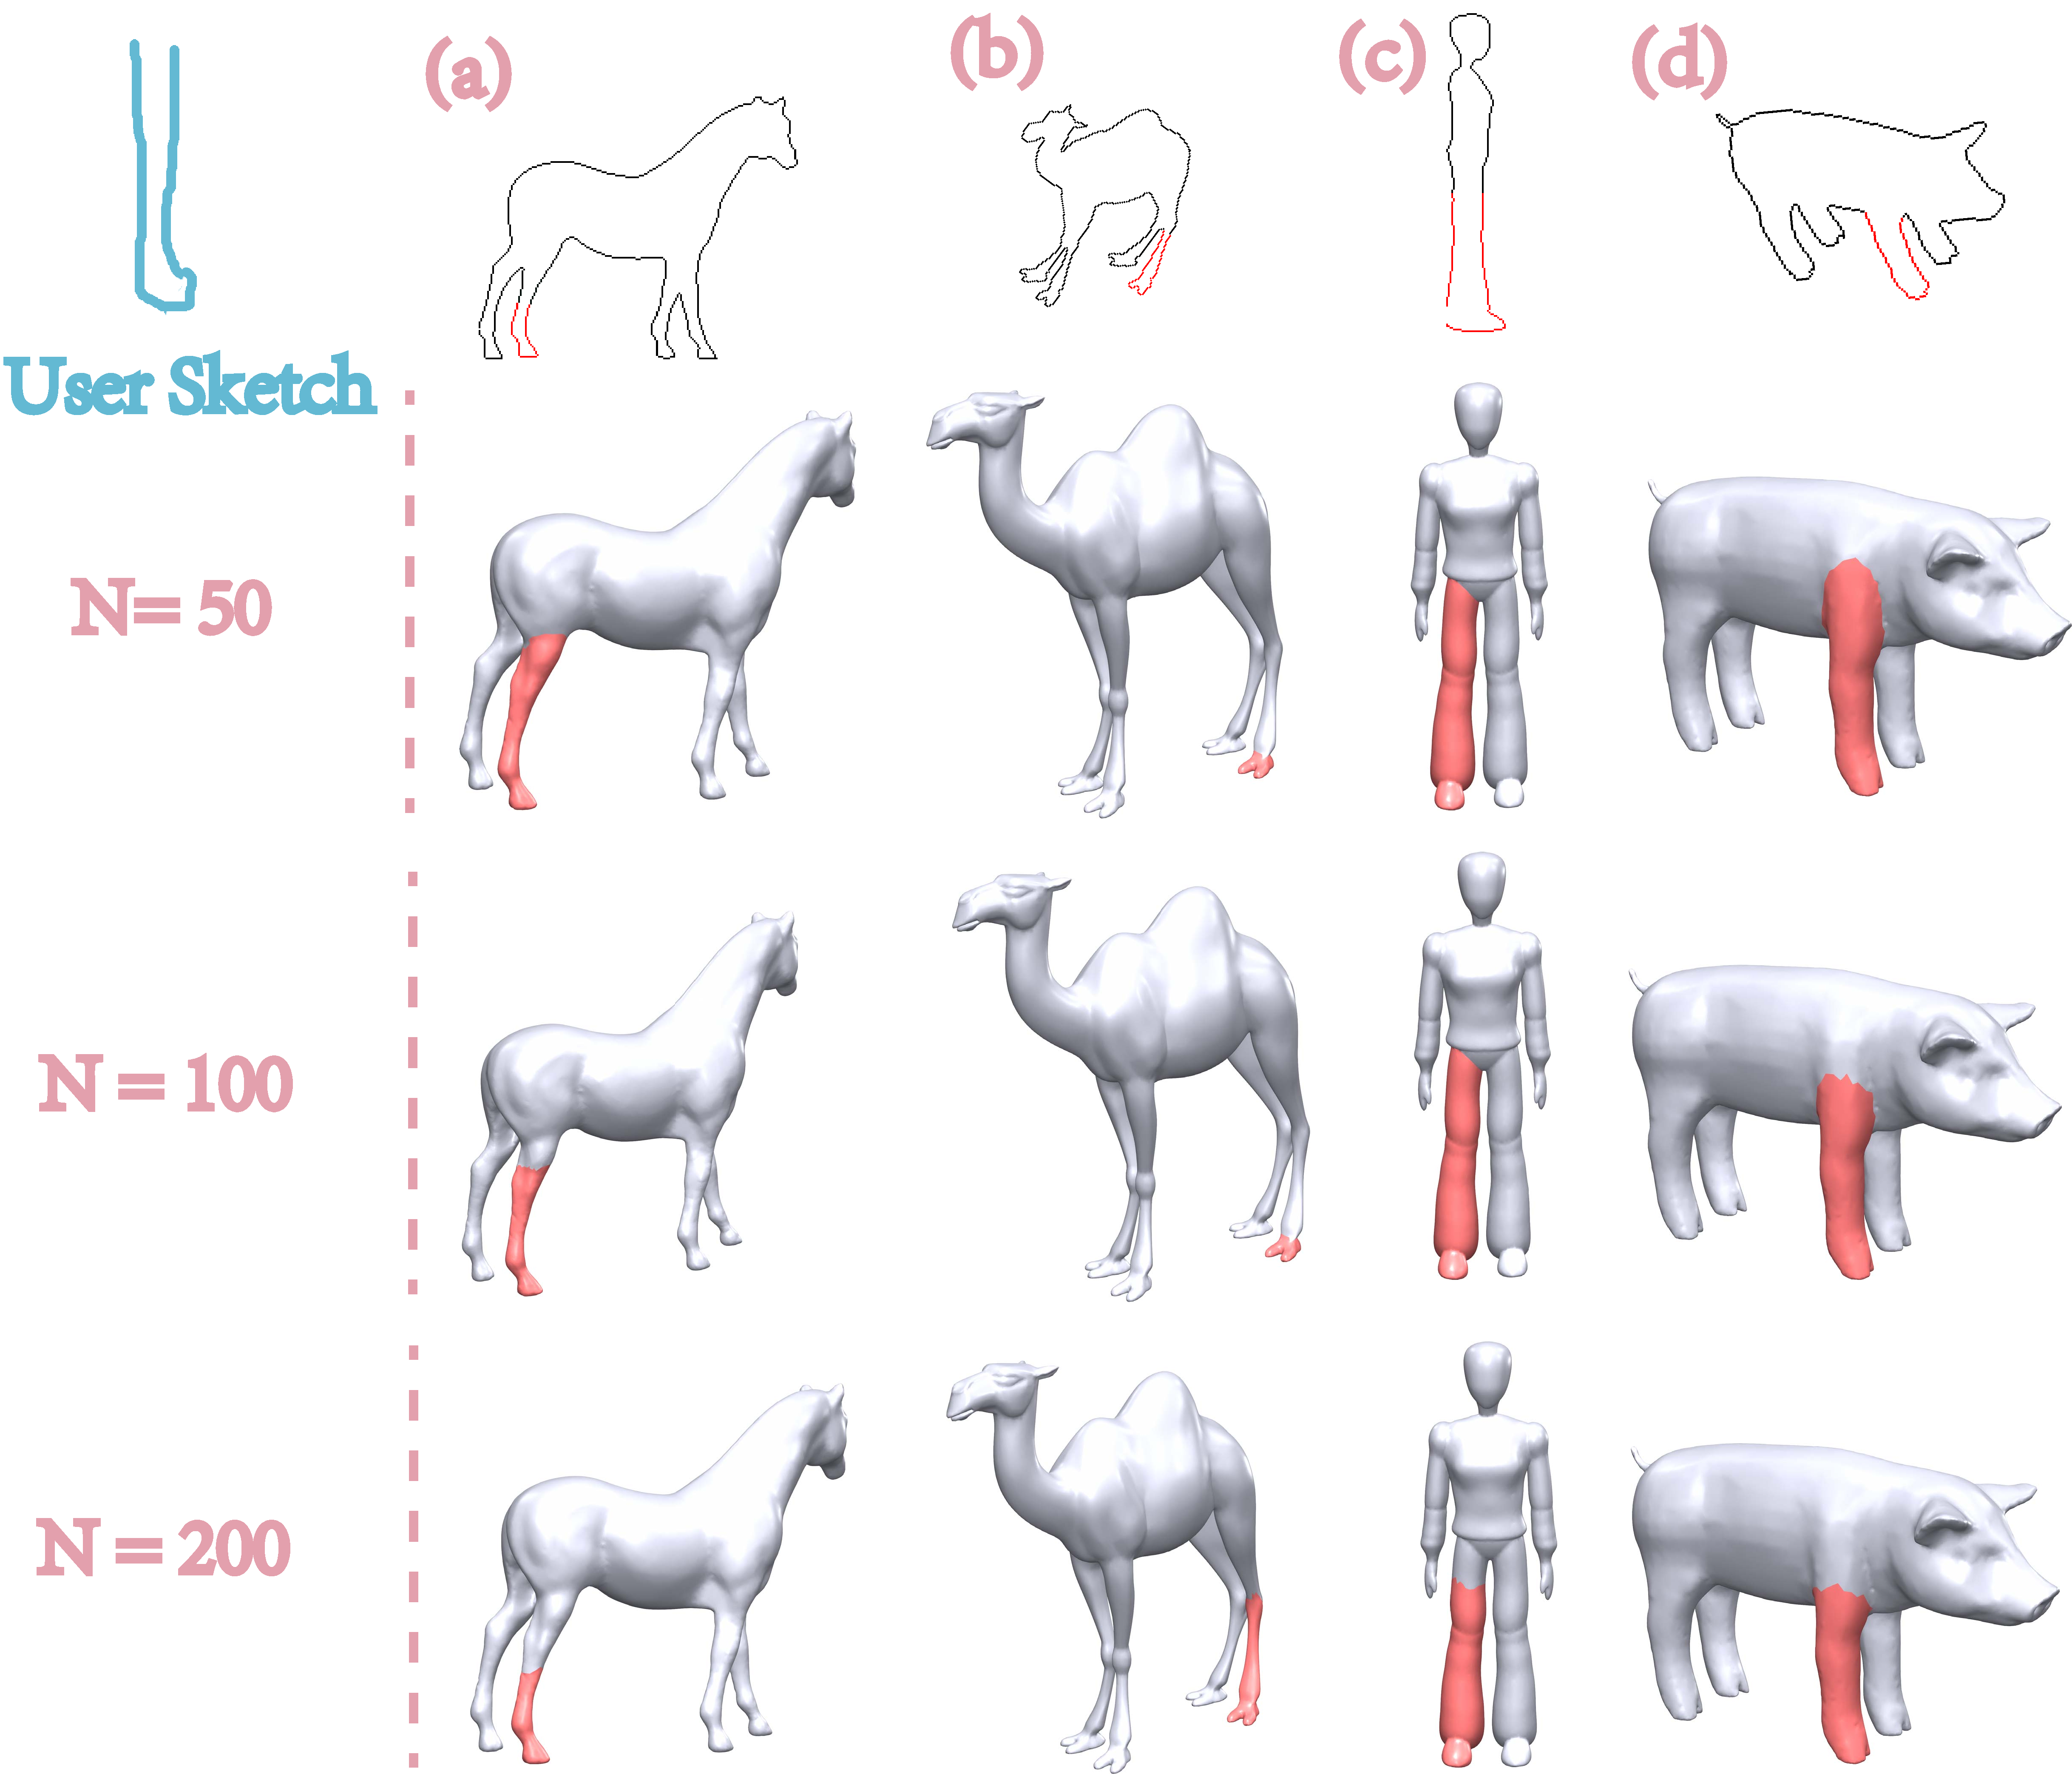
\includegraphics[width=1.0\linewidth]{./Material/SFGNVary.pdf}
\caption{Improvement in part quality with increasing super-face count (N). With more super-faces, the extracted part fits the user's sketch better and better.}
\label{fig:SFCountsPartQuality}
\end{figure}

\paragraph*{Comparison.}\hl{ We compare our method to the approach depending on the presegmented database (PreSeg). The PreSeg method is performed as follows: 1). Each database model is pre-segmented into regular (typical semantic) parts. For example, a human model is decomposed into four parts: head, torso, arms, and legs. 2). We extract boundary contours for each part under different camera views. 3). We construct the kNN graph for the part contours. The node in the kNN graph represents the complete part contour. The edge is established by global matching between part contours. 3). In the runtime stage, given the 3D proxy, a list of candidate parts are retrieved through a similar procedure as Ours with the only difference that contour matching is performed in a global manner. The matching error for the PreSeg method is 0.624 averaged over a set of 20 test sketches. Compared with Table }\ref{tab:MatchError}\hl{, our method clearly outperforms the PreSeg method. The visual result is shown in figure }\ref{fig:Comp2PreSeg}\hl{. Because our method generate candidate parts on-the-fly, the retrieved parts are more similar to the user sketch.}
%--------------------------
\begin{figure}\centering
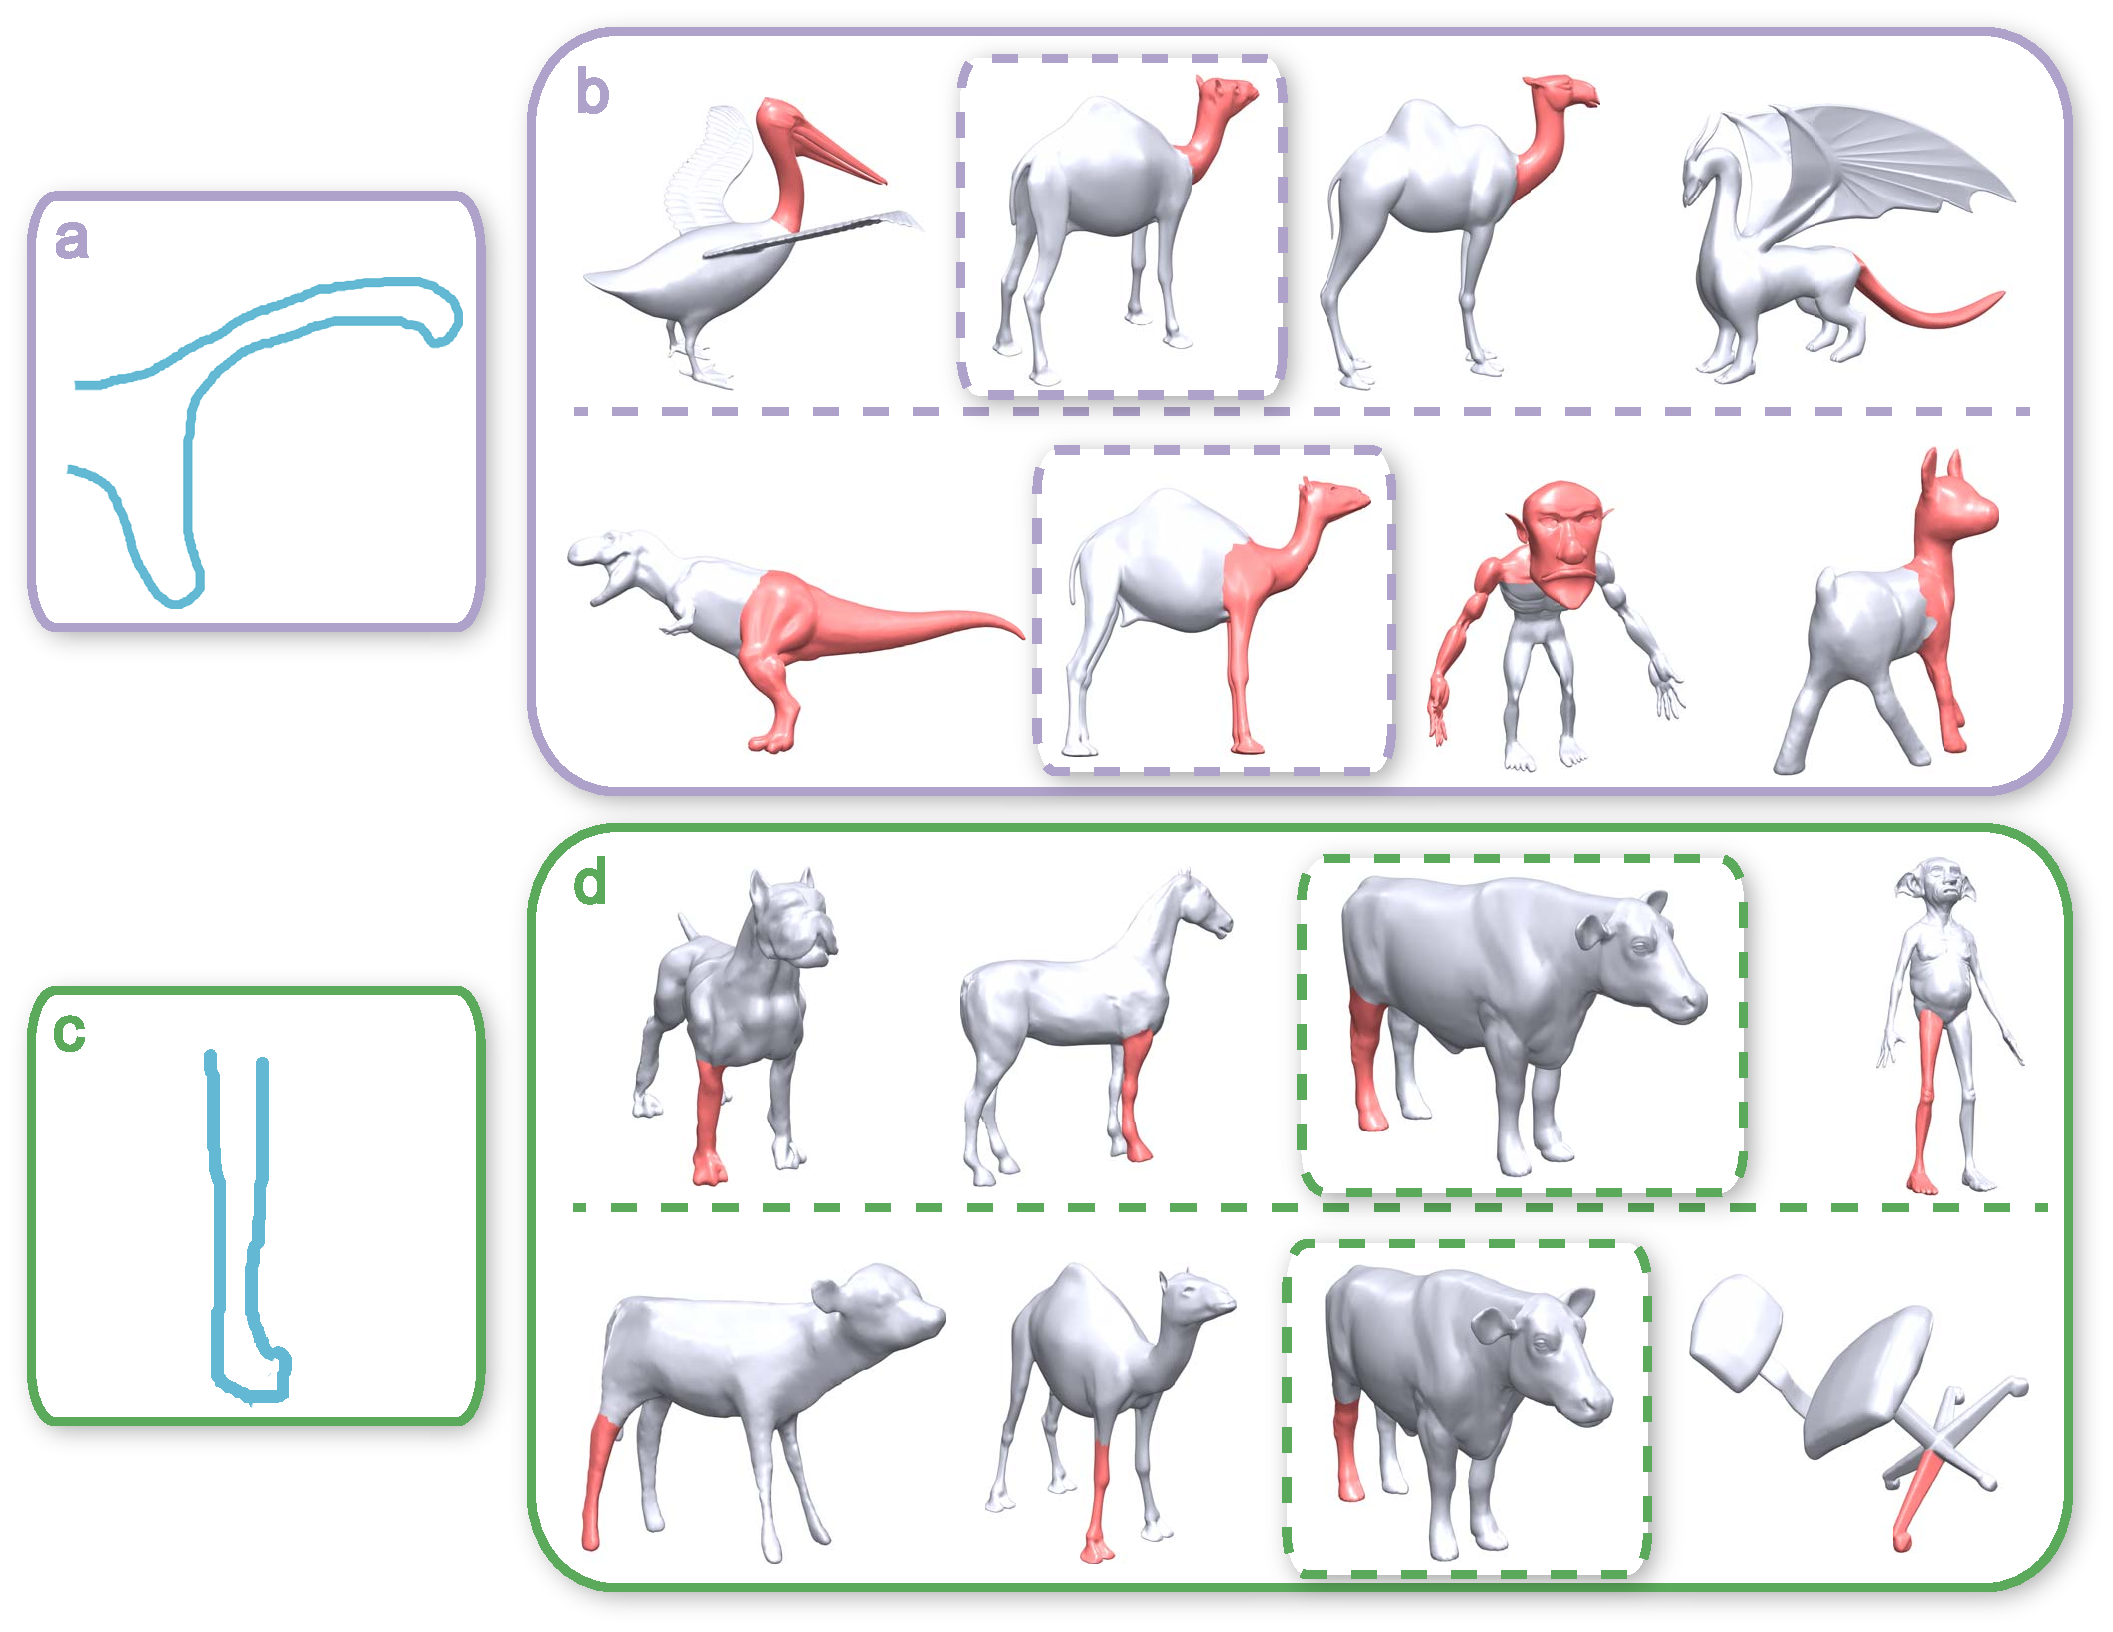
\includegraphics[width=1.0\linewidth]{./Material/Comp2PreSeg.pdf}
\caption{Retrieval results generate with our method and PreSeg method. Given the same sketch, we show the retrieval results generated with the two methods.
In (b) and (d), our results is on the upper row, the PreSeg results is on the lower row. Notice the results circled in (b) and (d), we could conclude that our method could generate candidate parts more similar to the user sketch.}\label{fig:Comp2PreSeg}
\end{figure}

\paragraph*{Camera views.} \hl{We have evaluated the influence of the camera views. Figure }\ref{fig:PreRecCurve}\hl{(b) shows the precision recall curve under different camera views. The 7 camera views include 3 canonical side views and 4 corner views. The other camera views include the 7 camera views and other uniformly sampled views}~\cite{FanWang2013}\hl{. To balance between efficiency and effectiveness, we use 21 views.} 


%%%%%%%%%%%%%%%%%%%%%%%%%%%%%%%%%%%%%%%%%%%%%%%%%%%%%%%%%%%%%%%%%%%%%%%%%%%%%%%%%%%%%%%%%%%%%%%%%%%%%%%%%%%%
\section{Conclusion}
We have introduced a sketch-based customized part extraction algorithm for 3D shape modeling. Our approach queries a database in real time and retrieves parts matching the user's sketch. In contrast to previous methods, our approach does not rely on a pre-segmented database. Instead, it generates customized parts on-the-fly to accurately match the sketch, thus significantly enriching the design space. Candidate parts are identified and segmented by a fast 2D-to-3D partial matching technique. Our algorithm enables several applications.

\textbf{Limitations.}  In our current implementation, we assume that the models in the database are manifold. Also, the contour descriptor we adopt is not scale-invariant.

\textbf{Future work.} We plan to develop more powerful scale-invariant contour descriptors. Since there have been several improvements to the angle descriptor~\cite{frompartialshapematchingcvpr}, we would like to incorporate these more powerful descriptors in our framework. In addition, it would be nice to incorporate cues from surrounding context to help disambiguate sketches.
\hl{Local symmetry/similarity matching could benefit from the context-based search.}
The view under which the sketch is drawn is important: some views are more discriminative than others. Helping users to draw optimal views and/or helping them interactively resolve ambiguous sketches, is an important research direction.
\hl{We plan to investigate the recognized definition of the partial matching problem in the future. }
\hl{It is also of interest to test our method in a more larger database. }
\hl{The fundamental premise of the sketch-based shape retrieval approaches is that the example database becomes larger by implicitly containing all possible segmented parts. We plan to investigate it in the future. }
\hl{The pose of the partial shape used for computing the boundary contours is important for our method.
If a suboptimal view is chosen, the method can return inappropriate candidate parts.
It would be interesting to explore the problem of best view selection in the future. } 

%%%%%%%%%%%%%%%%%%%%%%%%%%%%%%%%%%%%%%%%%%%%%%%%%%%%%%%%%%%%%%%%%%%%%%%%%%%%%%%%%%%%%%%%%%%%%%%%%%%%%%%%%%%%%
%\section*{Acknowledgements}
%Special thanks to Yutong Wang for the implementation of the 3D proxy construction. We also thank Kuan Wang, Tian Qiu, Wanxuan Sun, Yue Huang and Qianqian Ye for preparing the results; the reviewers for the constructive comments; Siwang Li, Xuan Cheng and Debing Zhang for suggestions on the suggestive contours matching algorithm. This research is is supported in part by grants from \ldots

%%%%%%%%%%%%%%%%%%%%%%%%%%%%%%%%%%%%%%%%%%%%%%%%%%%%%%%%%%%%%%%%%%%%%%%%%%%%%%%%%%%%%%%%%%%%%%%%%%%%%%%%%%%%
\bibliographystyle{eg-alpha}
%\nocite{*}
\bibliography{Bib}
\end{document}
